\documentclass[TOTEM]{cern/cernphprep}

\usepackage{color}
\usepackage{enumitem}
\usepackage{lineno}

%----------------------------------------------------------------------------

\def\d{{\rm d}}
\def\un#1{\,{\rm #1}}
\def\ung#1{\quad[{\rm #1}]}
\def\unt#1{[{\rm #1}]}
\def\e{{\rm e}}
\def\I{{\rm i}}
\def\T{{\rm T}}
\def\vec#1{\mathbf{#1}}
\def\mat#1{\mathsf{#1}}
\def\etal{et al.}
\def\todo#1{{\color{red}TODO: #1}}
\def\TODO#1{{\color{red}TODO: #1}}

\setbox123\hbox{$0$}
\setbox124\hbox{$.$}
\def\S{\hbox to\wd123{\hss}}
\def\.{\hbox to\wd124{\hss}}

\def\Name#1{#1, }
\def\Review#1#2#3#4{{\it #1} {\bf #2} (#3) #4}

\def\hang{\hangindent=\parindent}
\catcode`\>=11
\newskip\itskip \itskip2mm
\newskip\iitskip \iitskip0mm
\newdimen\itindent \itindent3mm
\newdimen\iitindent \iitindent5mm
\def\>{\par\vskip\itskip\parindent\itindent\indent\hang\llap{\hbox to3mm{$\bullet$\hss}}}
\def\>E{\par\vskip\itskip\parindent\itindent\indent\hang\llap{\hbox to3mm{\hss}}}
\def\>>{\par\vskip\iitskip\parindent\iitindent\indent\hang\llap{\hbox to\iitindent{\hss--\ }}}

%----------------------------------------------------------------------------------------------------

\begin{document}

\begin{titlepage}

\renewcommand{\EXPLOGO}{fig/logo_totem_black.pdf}

\PHnumber{TODO}
\PHdate{TODO}

\EXPnumber{TODO}
\EXPdate{TODO}

\title{Alignment of CT-PPS detectors in 2016, before TS2}

\ShortTitle{Alignment of CT-PPS detectors in 2016}

\author{Jan Ka\v spar}

\ShortAuthor{Jan Ka\v spar}

\begin{abstract}
This note presents the first alignment of the CMS-TOTEM Precision Proton Spectrometer (CT-PPS) using the data from before Technical Stop 2 (TS2), 2016. This new procedure involves two stages. In the first one, data from a special calibration fill are used. In this fill, both horizontal and vertical Roman Pots (RPs) were inserted very close to the beam. In the second stage, hit distributions from physics fills (with only horizontal RPs inserted) are matched to the previously aligned reference from the calibration fill. The alignment and optics calibration is verified by reconstructing consistent $\xi$ spectra from different RPs and LHC fills.
\end{abstract}

%\centerline{version 0}	% sent on 19 Dec 2016
\centerline{version 2}

\end{titlepage}

%----------------------------------------------------------------------------------------------------

\linenumbers

\section{Introduction}
\label{s:intro}

Proper alignment is obviously important for physics reconstruction. For CT-PPS, therefore, horizontal alignment is of primary importance as it directly contributes to the reconstruction of proton momentum loss, $\xi$. To estimate the precision needed, one can consider another reconstruction uncertainty: the uncertainty of the horizontal dispersion, $D_x$. Taking the relative uncertainty of $5\un{\%}$ \cite{optics_calibration} and typical values $D_x \approx 8\un{cm}$ and $\xi \approx 0.05$ yields a horizontal hit position uncertainty of $200\un{\mu m}$.

Figure~\ref{fig:rp_layout} shows the layout and naming scheme \cite{rp-names} of the RPs around IP5. The RPs marked in red are used by CT-PPS and will be of primary interest of this note. The vertical RPs in both $210\un{m}$ stations are also used for alignment purposes.

\begin{figure}[h!]
\begin{center}
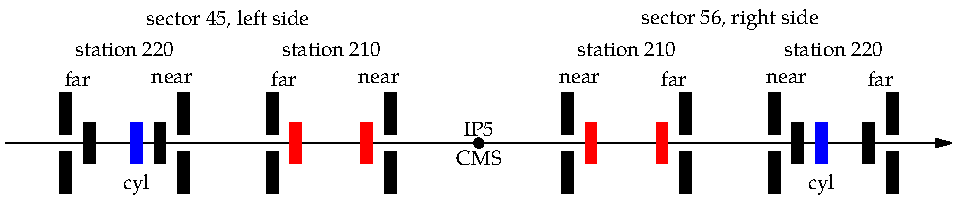
\includegraphics{fig/rp_layout.pdf}
\caption{%
Layout of RPs around IP5. The red RPs contain the tracking Si strips sensors used for CT-PPS. The blue (cylindrical) RPs host the timing diamond sensors. The other RPs are used by the TOTEM experiment.
}
\label{fig:rp_layout}
\end{center}
\end{figure}

This note describes the first alignment of CT-PPS data taken in 2016, before TS2 -- in the LHC fills 4947 through 5288. 

The alignment proceeds in the following two stages.
\begin{enumerate}[nosep]
\item Alignment is performed with data from a special low-luminosity calibration fill (4828), where both horizontal and vertical RPs are inserted very close to the beam (about $5\un{\sigma}$). The standard TOTEM procedure \cite{totem-ijmp} is used, details will be given in Section~\ref{s:calib}.
\item The alignment information is transferred from the calibration fill to the standard physics fills with high luminosity and only horizontal RPs inserted. This new procedure is described in Section~\ref{s:phys}.
\end{enumerate}

The alignment and optics calibration \cite{optics_calibration} is eventually followed by a reconstruction validation, see Section~\ref{s:val}.

This article uses a reference frame where $x$ denotes the horizontal axis (pointing out of the LHC ring), $y$ the vertical axis (pointing against gravity) and $z$ the beam axis (in the clockwise direction).


%----------------------------------------------------------------------------------------------------

\section{Alignment in calibration fill}
\label{s:calib}

This stage is performed with a special LHC fill, sometimes called ``alignment fill''. This fill can be characterised by low beam intensity, both horizontal and vertical RPs inserted and all RPs being close to the beam (about $5\un{\sigma}$).

The standard ``TOTEM'' alignment, see Section 3.4 in \cite{totem-ijmp}, is applied. It can be summarised by the following three steps.
\begin{enumerate}[nosep]
\item {\em Beam-based alignment} -- a procedure which takes place before data-taking and the purpose of which is to align the RPs with the LHC collimators and the beam. For that collimators scrape the beam to have a sharp edge and then each RP is slowly approached until a contact with the beam is signalised by a spike in beam-loss monitors downstream (see Figure 7 in \cite{totem-ijmp}). At this point, the RP is at the same $n_\sigma$ distance as the collimator which defines its position, used as a starting point for the alignment.
\item {\em Relative alignment among RPs} is achieved by analysing residuals between hits and track fits within each RP station. In this step, position (shift in the read-out direction) and rotation (about the beam axis) of each Si sensor is optimised. Thanks to the overlap between the horizontal and vertical RPs, see Figure~\ref{fig:rp_overlap}, the relative position among all sensors within a station can be determined. Details of the procedure are given in Section 4.2 in \cite{jan_thesis}, the application to the present data is described in Section~\ref{s:calib-track}.
\item {\em Absolute alignment wrt.~the beam} is performed with a sample of elastic-scattering events tagged by the vertical RPs. Due to the azimuthal symmetry of the process, the position of the beam can be derived from the observed hit distributions. For more details see Section~\ref{s:calib-elastic}.
\end{enumerate}

%--------------------------------------------------
\subsection{Relative alignment among RP sensors}
\label{s:calib-track}

This step uses the method presented in Section 4.2 in \cite{jan_thesis} based on analysis of the residuals between hits and track fits. While any track passing through a RP station can be used, the most valuable tracks are those passing through several RPs. The key point of the method is the overlap between the horizontal and vertical RPs as shown in Figure~\ref{fig:rp_overlap}, which allows to determine the relative alignment among all sensors of a station.

\begin{figure}[h!]
\begin{center}
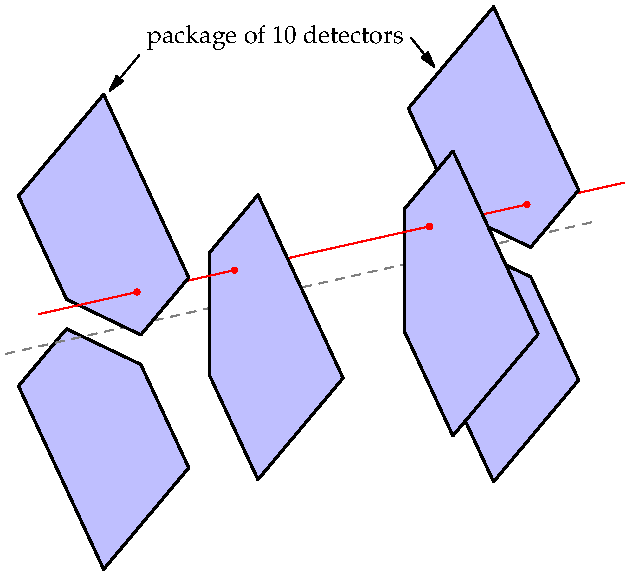
\includegraphics[width=5cm]{fig/rp_overlap.pdf}
\caption{%
A track (red line) passing through an overlap between vertical and horizontal RPs. The blue areas represent stacks of 10 Si strip sensors. The dashed black line indicates the beam.
}
\label{fig:rp_overlap}
\end{center}
\end{figure}

The procedure optimises the shift (in read-out direction, i.e.~perpendicular to strips) and rotation (about beam axis) of each sensor. The optimisation is performed in 5 iterations, gradually imposing more strict track building cuts as alignment precision improves. Typically, only tracks with hits in at least 3 RPs are used -- to prevent building tracks from unrelated hits.

Obviously, this method is not sensitive to misalignment modes which do not induce residuals. These include global shifts and rotations and will be addressed by the next step, see Section~\ref{s:calib-elastic}. In order to find a unique solution in this step, the optimisation is performed with the constraint of zero global alignment corrections.

The method is applied separately to several data sub-samples (different TOTEM runs) in order to verify the stability of results and gain control over the systematics.

Note that the method works even without the RP 56-210-nr-tp which did not send data due to technical problems.

Figure \ref{fig:tb_residuals} shows examples of residual distributions in several phases of the optimisation. As expected, during the optimisation the width of the distributions decreases and the originally disconnected portions (coming from various RP combinations) become all centred around zero. The final width of the residual distribution is compatible with the sensor pitch of $66\un{\mu m}$.


\begin{figure}[h!]
\begin{center}
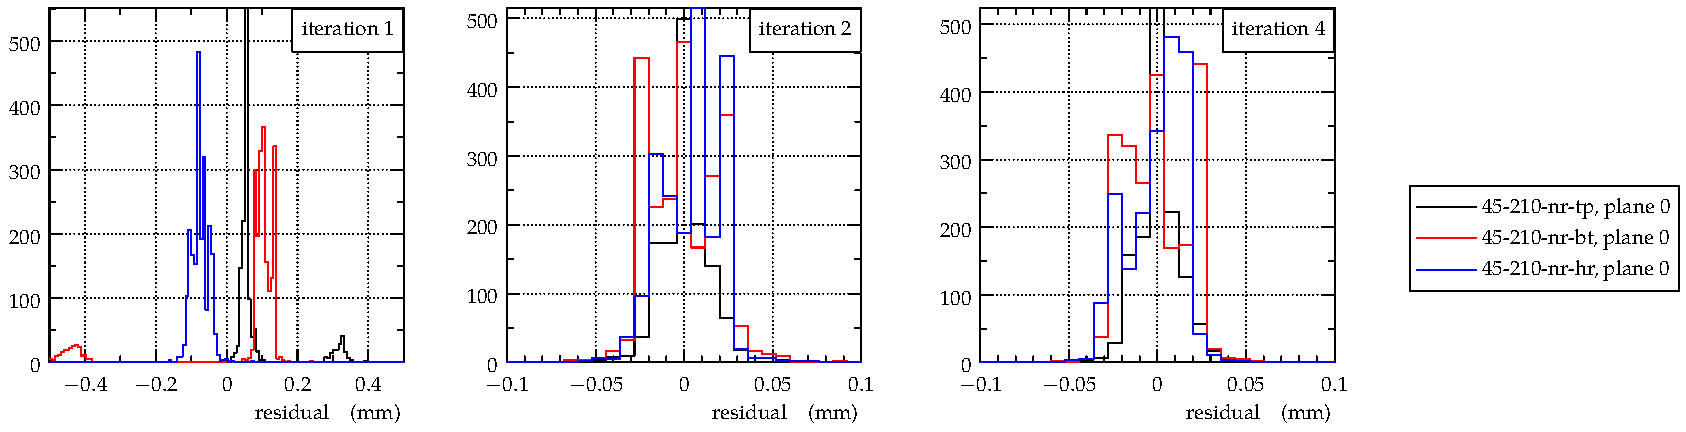
\includegraphics[width=\hsize]{fig/calibration_fill/residuals.pdf}
\caption{%
Distributions of track-hit residuals (TOTEM run 10079). Each colour corresponds to a different sensor (first planes in the RPs of the 45-210-nr unit). The blue histogram in the left plot has been downscaled by factor 100. {\it Left}: before any optimisation. The disconnected histogram portions originate from different RP configurations contributing to the track fit. {\it Middle}: after shift optimisation. {\it Right}: after shift and rotation optimisation.
}
\label{fig:tb_residuals}
\end{center}
\end{figure}

The results of this alignment step may be conveniently decomposed into ``RP alignments'' -- alignments shared by all sensors in a RP -- and ``internal alignments'' -- sensors alignments wrt.~the RP alignments.

Figure \ref{fig:tb_example_internal} shows an example of the ``internal alignments''. The agreement between the different colours representing different data samples demonstrates the stability of the procedure. The linear patterns in the determined shifts (separately in ``U'' and ``V'' projections) can be understood by tilts of the entire detector package which shift the sensor's centre proportionally to its position within the package, for more details see Section 4.2.8 in \cite{jan_thesis}.

\begin{figure}[h!]
\begin{center}
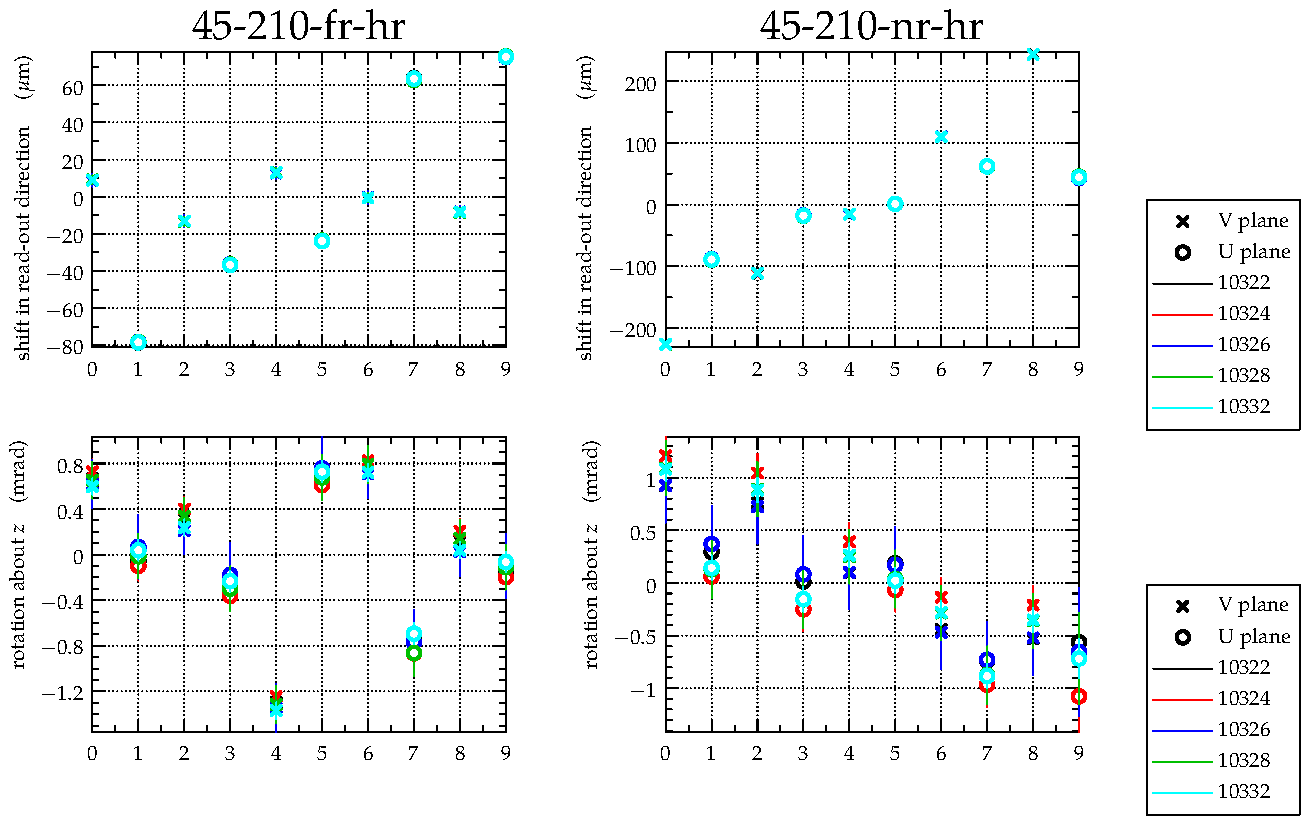
\includegraphics[width=0.8\hsize]{fig/calibration_fill/plots_per_plane_left.pdf}
\caption{%
Comparison of the ``internal alignments'' obtained from different TOTEM runs (different colours). The two columns correspond to the two horizontal RPs in the sector 45. The horizontal scale gives the plane index within the detector package: 0 is the closest to the IP, 9 the farthest. The results for ``V'' (``U'') planes are marked with crosses (circles). The error bars indicate statistical uncertainties only.
}
\label{fig:tb_example_internal}
\end{center}
\end{figure}

Figure \ref{fig:tb_example_rp} shows a summary of the determined ``RP alignments''. There is a good agreement among the results obtained from different data sub-samples.

\begin{figure}[h!]
\begin{center}
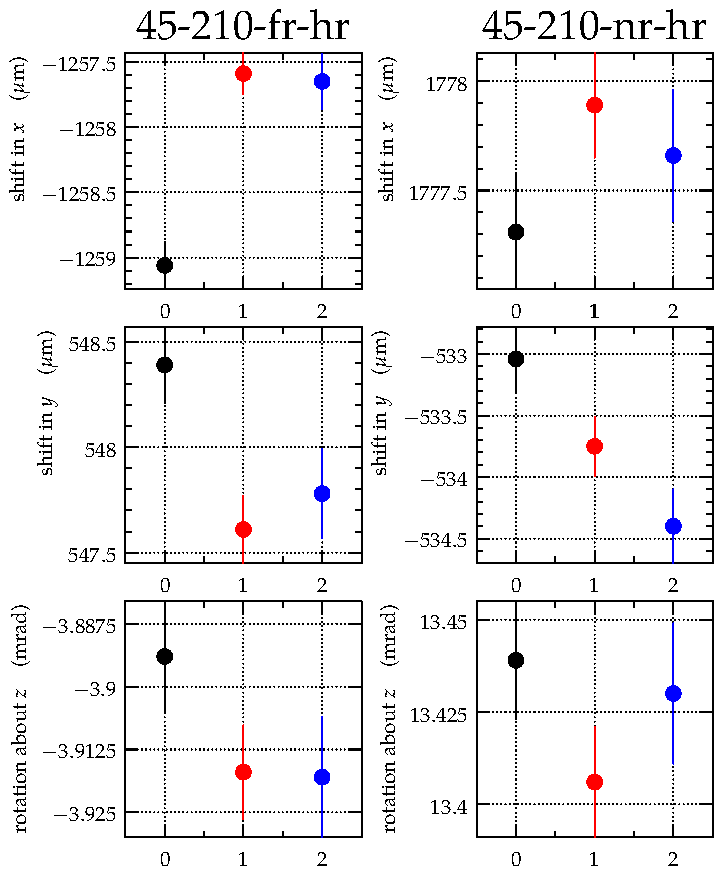
\includegraphics[height=8.5cm]{fig/calibration_fill/plots_per_rp_left.pdf}
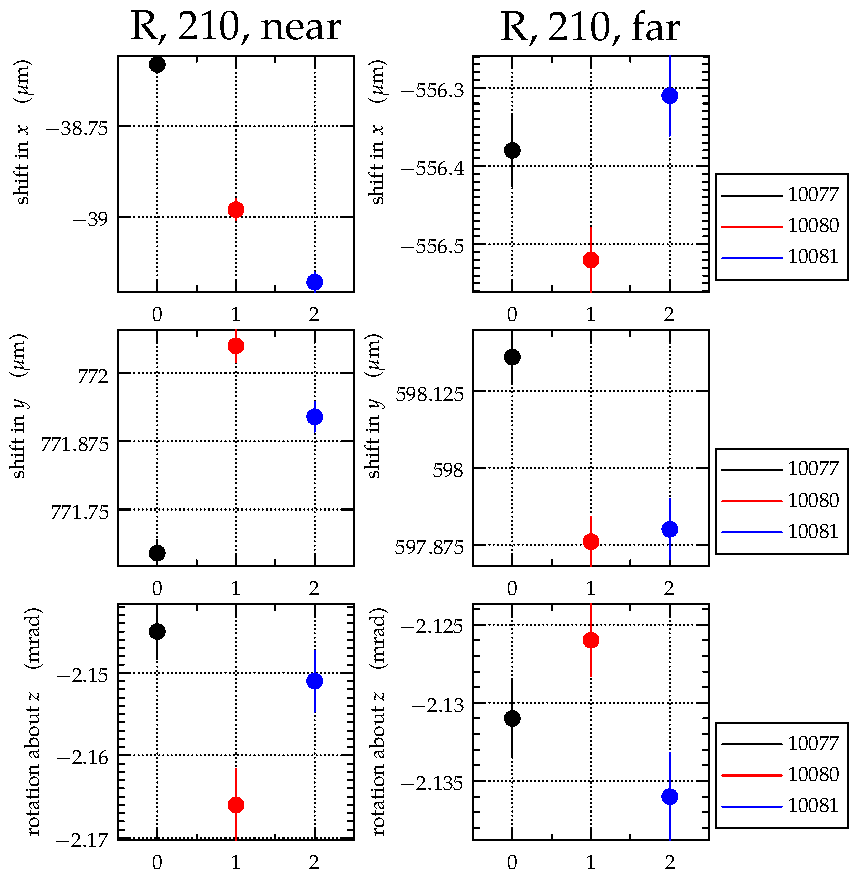
\includegraphics[height=8.5cm]{fig/calibration_fill/plots_per_rp_right.pdf}
\caption{%
Comparison of the ``RP alignments'' obtained from different TOTEM runs (different colours). Each column corresponds to one horizontal RP, each row represents an alignment parameter. The error bars indicate statistical uncertainties only.
}
\label{fig:tb_example_rp}
\end{center}
\end{figure}

The statistical component of the alignment uncertainties is estimated by the algorithm. The systematic component can be inferred from the difference between the sub-samples, cf.~Figures \ref{fig:tb_example_internal} and \ref{fig:tb_example_rp}. A conservative estimate of the combined uncertainties is $3\un{\mu m}$ for shifts, $0.2\un{mrad}$ for rotations.


%--------------------------------------------------
\subsection{Absolute alignment with respect to the beam}
\label{s:calib-elastic}

This step exploits the azimuthal symmetry of elastic scattering. This process has a large cross-section and is relatively easy to tag due to the two (almost) anti-parallel protons in the final state. Taking into account the LHC optics, the elastic hit distribution in any RP has elliptical contour lines around the beam position. This symmetry is used in an analysis of the detected hit distributions in order to determine the beam location wrt.~the RP sensors.

Due to the properties of the LHC optics, the elastic tracks are detected in the vertical RPs. Compared to standard elastic tagging (e.g.~Section~5.2.1~in \cite{totem-8tev-90m}), this dataset presents a complication due to missing RP 56-210-nr-tp, which comes with two consequences. First, the horizontal scattering angle ($\theta_x^*$) cannot be reconstructed in optimal way -- using both near and far RPs, optimising both resolution and stability against optics imperfections. Second, since only 1 RP can be used for reconstruction in the right arm (and the affected diagonal), only 1 kinematic variable can be reconstructed: $\theta_x^*$. As the horizontal vertex position, $x^*$, is not determined the number of tagging cuts is reduced.

The elastic-selection cuts include
\begin{itemize}[nosep]
\item $\theta_x^*$ left-right collinearity, see Figure \ref{fig:el_cuts}, top left,
\item $\theta_y^*$ left-right collinearity, see Figure \ref{fig:el_cuts}, top right,
\item $x^*$ in the left arm compatible with vertex distribution, see Figure \ref{fig:el_cuts}, bottom left,
\item position-angle correlation in $y$ plane in the left arm, see Figure \ref{fig:el_cuts}, bottom right.
\end{itemize}

\begin{figure}[h!]
\begin{center}
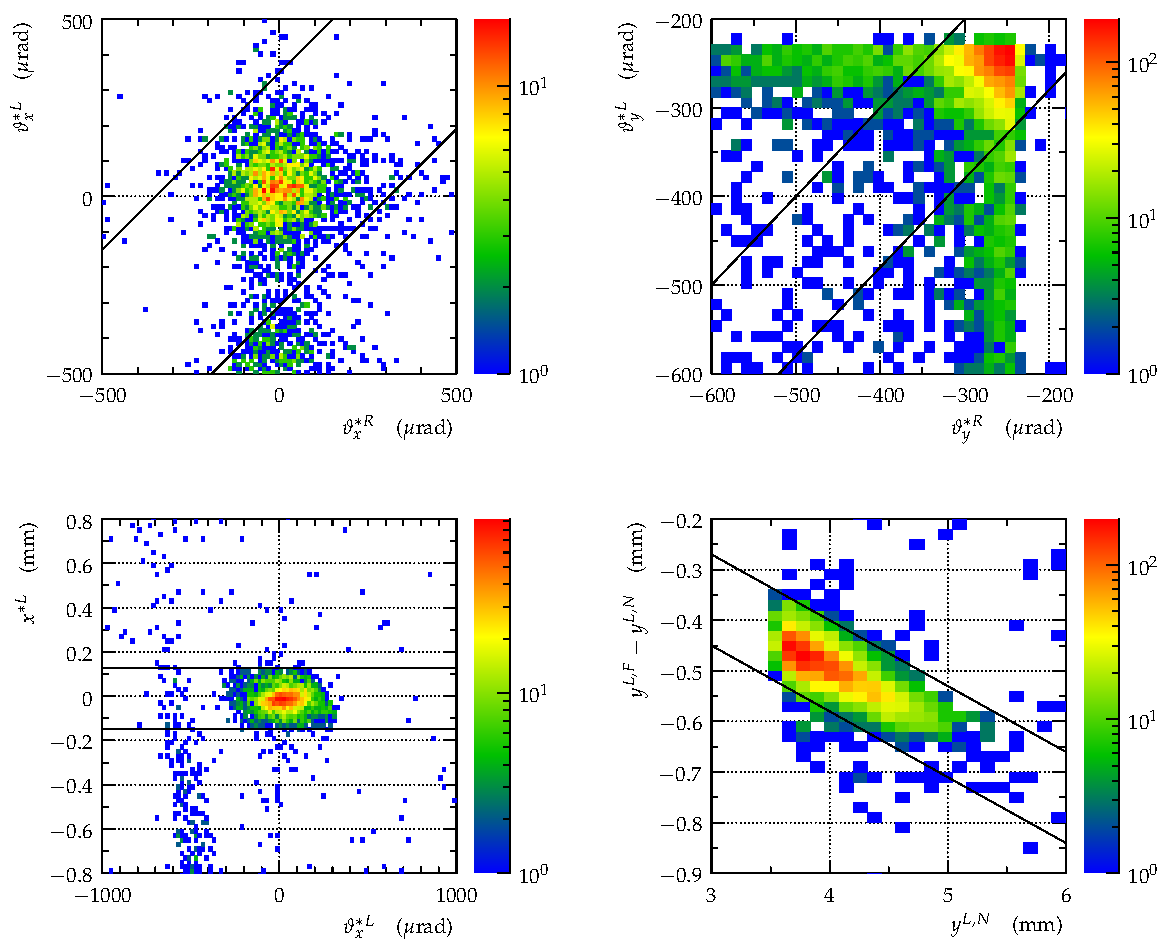
\includegraphics[width=1\hsize]{fig/calibration_fill/el_cut_example.pdf}
\caption{%
Example of elastic selection cuts. The black lines delimit the selection region. $\theta_x^*$ and $\theta_y^*$ represent the horizontal and vertical scattering angles. $x^*$ denotes the horizontal vertex positions. In the superscripts, L stands for left (sector 45), R for right (sector 56), N for near and F for far.
}
\label{fig:el_cuts}
\end{center}
\end{figure}

\begin{figure}[h!]
\begin{center}
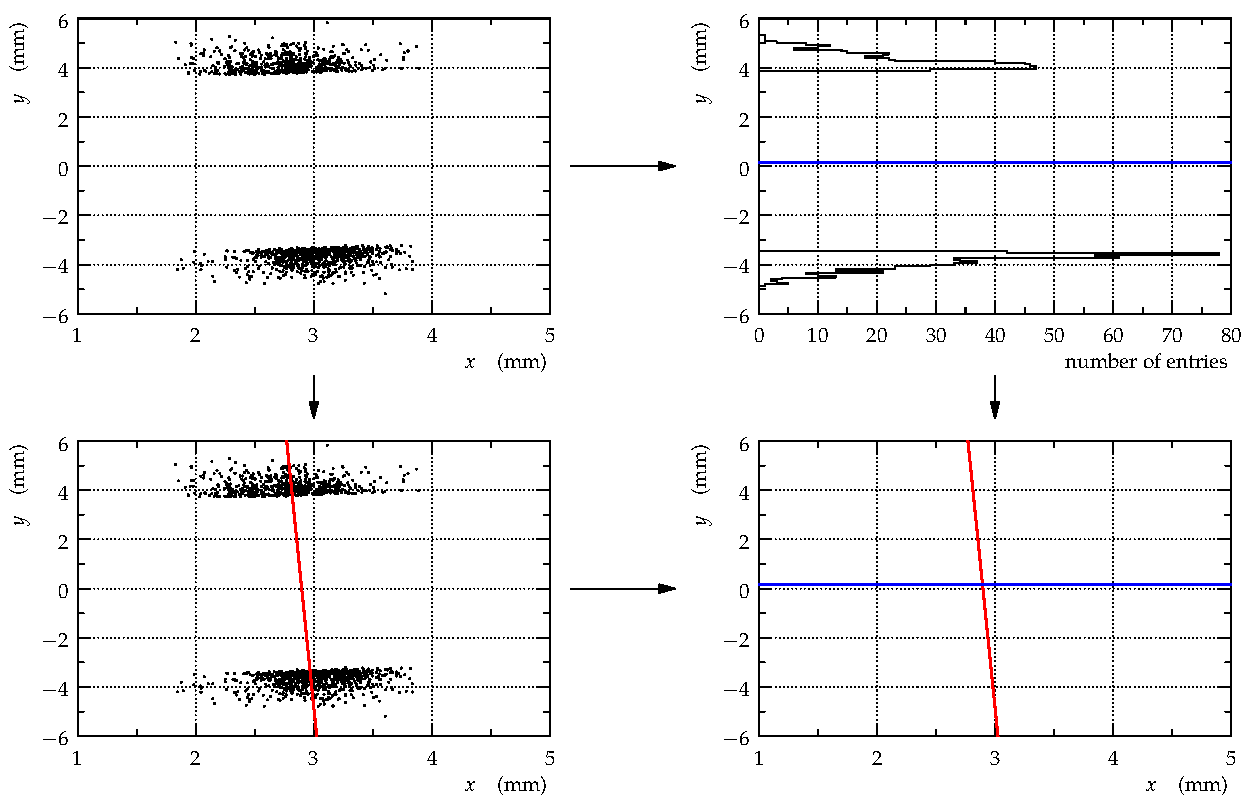
\includegraphics[width=1\hsize]{fig/calibration_fill/el_alignment_method.pdf}
\caption{%
Illustration of alignment with elastic-scattering hit distributions, using a 1h-slice of data. See text for description.
}
\label{fig:el_alignment_method}
\end{center}
\end{figure}

The alignment method is illustrated in Figure~\ref{fig:el_alignment_method}. The top left plot shows a hit distribution in a unit, the upper (lower) part comes from the top (bottom) RP. This distribution is fitted and a vertical axis is obtained, see the red line in the bottom left plot. Several fitting techniques are applied, including fitting a profile histogram and a $\chi^2$-based fit minimising the distance to all hits, dynamically down-weighting outliers. Both fit techniques give compatible results. In a next step, the vertical centre of the distribution is obtained, see the blue line in the top right plot. A non-parametric methods is used: the histogram part from the bottom RP is flipped around zero and then shifted up and down until the best match with the histogram from the top RP is found. For more details see Method 2 in Section 4.4 in \cite{jan_thesis}. Several matching metrics are considered, including $\chi^2$ and Kolmogorov-like expressions, all giving compatible results. Finally, the crossing of the blue and red lines indicates the position of the beam.

An exceptional approach had to be adopted for the unit 56-210-nr, where the data from the top RP were not available. First, the slope of the vertical axis (red line in Figure~\ref{fig:el_alignment_method}) was fixed to a value compatible with the one in the far RP. The dominant contribution of these slopes is expected to come from the $x$-$y$ coupling in the optics and thus very similar between the near and far RP. Second, the vertical alignment could not have been determined. An alternative method is available but was not applied: imposing the equivalence of $\theta_y^*$ reconstructed in all the 4 RPs measuring the same elastic event.

The alignment procedure was applied separately on 1h time slices of the data, in order to examine time variation and to control systematic effects. The results are summarised in Figure~\ref{fig:el_alignment_results}. Within tolerance, the time dependence can be considered as flat, with some measurements being obvious outliers. Consequently, the results can be reduced to a single value per RP and variable, see the solid red lines in the figure.

\begin{figure}[h!]
\begin{center}
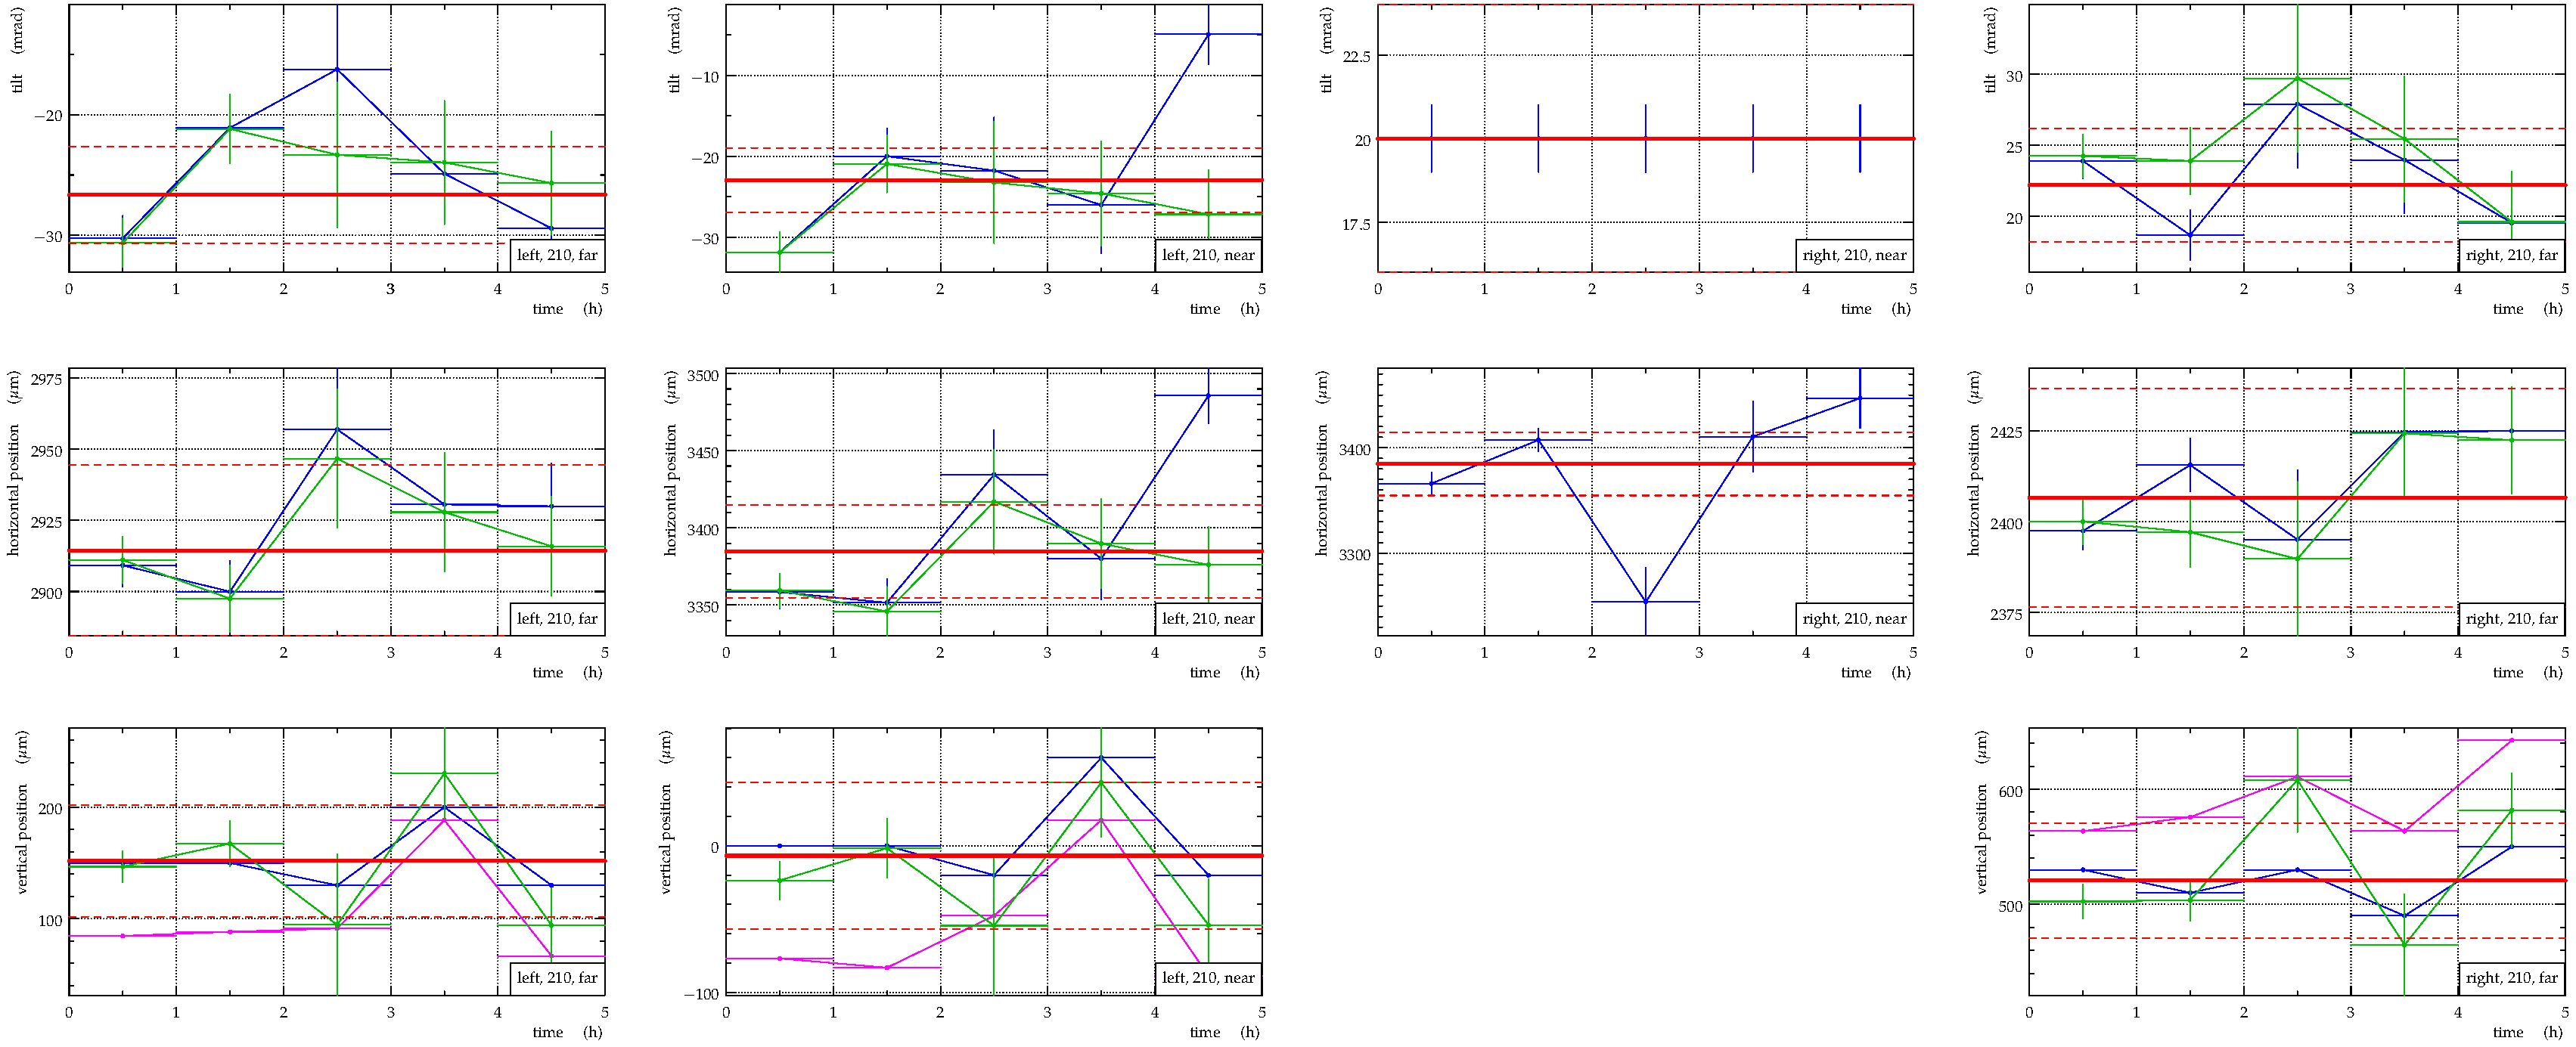
\includegraphics[width=\hsize]{fig/calibration_fill/el_alignment.pdf}
\caption{%
Summary of the elastic-alignment results. Each column corresponds to one RP unit. The rows (top to bottom) show: tilt (about the beam axis), horizontal beam position and vertical beam position. The error bars indicate statical uncertainties only. The horizontal axis gives time in hours since the beginning of the run. The red solid (dashed) lines denote the final extracted values (their uncertainties).
}
\label{fig:el_alignment_results}
\end{center}
\end{figure}

The uncertainties can be estimated from Figure~\ref{fig:el_alignment_results}. The statistical component is indicated by the error bars, the variation between the time slices indicates the systematic component. Altogether, a conservative uncertainty estimate is $5\un{mrad}$ for tilts, $50\un{\mu m}$ for horizontal shifts and $75\un{\mu m}$ for vertical shifts, as indicated by the red dashed lines in the figure.

%----------------------------------------------------------------------------------------------------

\section{Alignment in physics fills}
\label{s:phys}

In comparison to the calibration fill, the physics fills can be characterised by high intensity and only horizontal RPs inserted. Consequently a different alignment strategy had to be developed. The procedure is data-driven for both horizontal and vertical alignment and therefore it is important to verify the stability of the LHC conditions (beam orbit, position of collimators, etc.) -- see Section~\ref{s:phys-conditions}.

The horizontal alignment is based on the fact that the physics is the same in all fills. If the LHC conditions were stable, the same is true for the hit distributions observed in the RPs. Therefore, the alignment can be achieved by matching the hit distributions from a physics fill to the previously aligned hit distributions from the calibration fill. This method is detailed in Section~\ref{s:phys-horizontal}. For this method, it is obviously important to suppress non-physical background. A set of such cuts will be presented in Section~\ref{s:phys-data_selection}.

The vertical alignment is, in principle, simpler as the vertical beam position can be inferred from the maximum of the $y$ distribution which is within the acceptance of the horizontal RPs. See Section~\ref{s:phys-vertical} for details.

Regarding the RP position, there were two types of insertions within the period under study. In all fills the target position was $15\un{\sigma}$, in fills 4947, 4953, 4961, 4976 and a part of fill 4964 an additional safety margin of $0.5\un{mm}$ was applied. A graphical illustration is available in Figure~\ref{fig:cond_rp}.

%--------------------------------------------------
\subsection{Conditions}
\label{s:phys-conditions}

Figure~\ref{fig:cond_rp} presents a summary of the RP insertions over the period of interest. It shows the readings from the 3 position sensors after the RPs have been moved to the data-taking positions. The ``motor'' sensor counts the steps of the motor which moves the RP by turning a precision screw. This sensor has a precision of few micrometres, but depends on the calibration of the zero of its scale. The ``resolver'' measures the rotation of the screw. The ``LVDT'' (linear voltage differential transformer) gives a measurement that does not depend on any calibration procedure but is known to be subject to various drifts (due to temperature etc.). The figure shows that ``motor'' and ``resolver'' readings were always identical, the ``LVDT'' was compatible with them within its uncertainty. Moreover, the insertion position was stable over the period, as expected.

\begin{figure}[h!]
\begin{center}
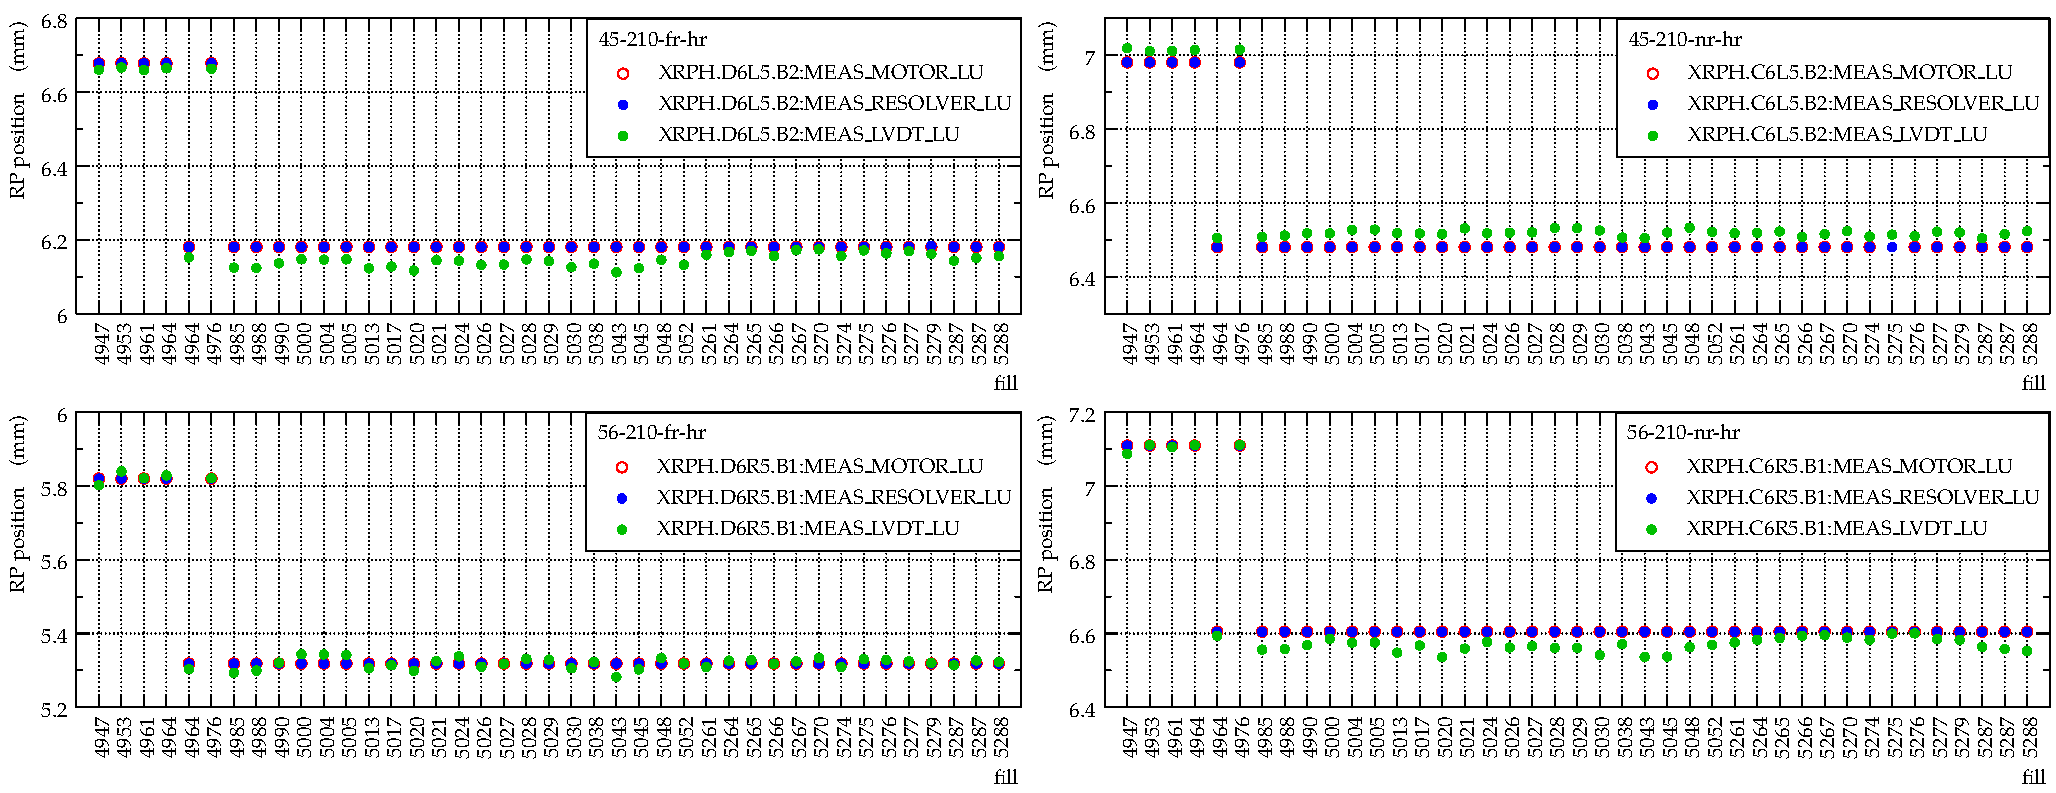
\includegraphics[width=1\hsize]{fig/conditions/rp_positions_rps.pdf}
\caption{%
RP positions as reported by the 3 position sensors (LVDT, MOTOR and RESOLVER) per LHC fill (horizontal axes). The two entries for fill 4964 correspond to the insertions with and without the safety margin. The two entries for fill 5287 correspond to the two insertions within the same fill.
}
\label{fig:cond_rp}
\end{center}
\end{figure}


Since the observed hit distributions reflect the relative position between RPs and the beam, it is important to verify the stability of the beam orbits, too. As shown in Figure~\ref{fig:cond_bpm}, the readings from beam-position monitors (BPMs) in beam 2 can be considered as time-independent, taking into account their uncertainty of about $~0.5\un{mm}$. The same conclusion can be drawn for beam 1.

\begin{figure}[h!]
\begin{center}
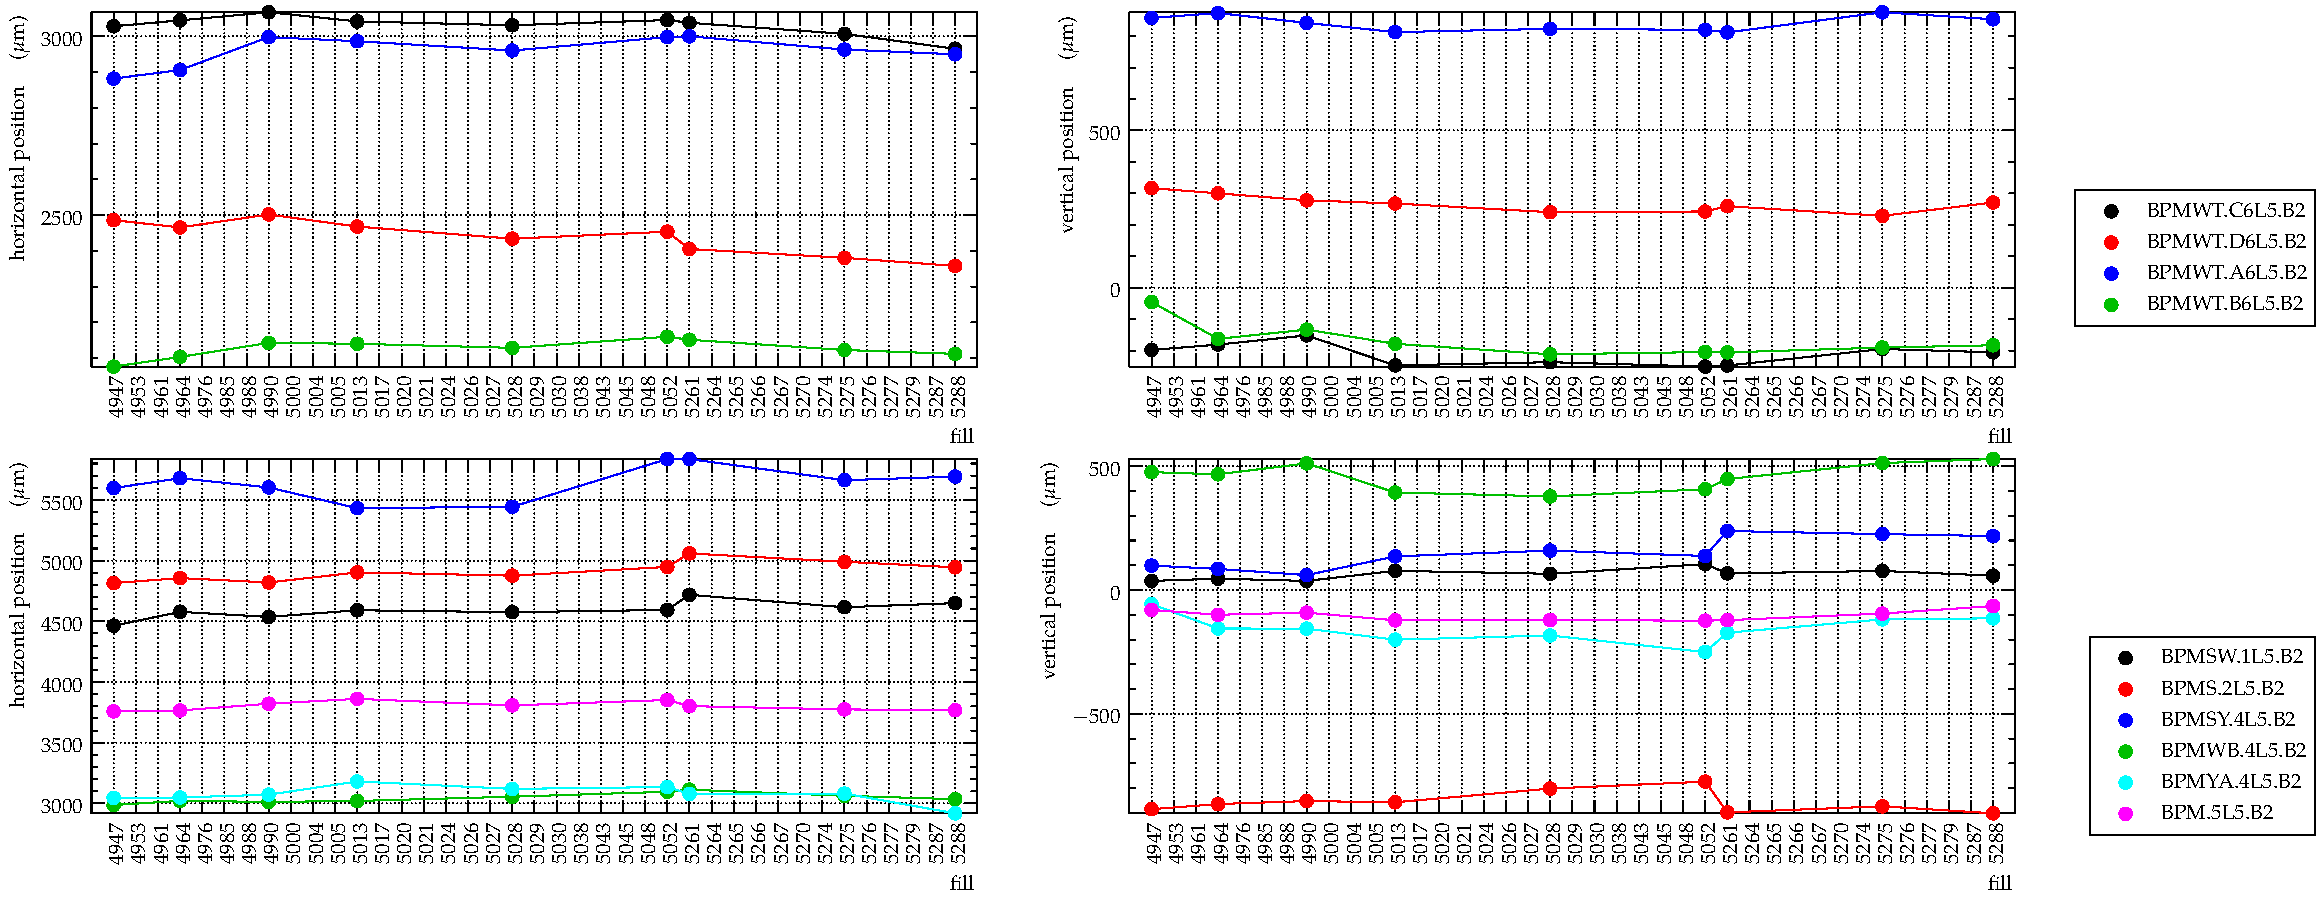
\includegraphics[width=1\hsize]{fig/conditions/bpm_comparison.pdf}
\caption{%
Readings of selected BPMs in beam 2 and between IP5 and the RPs, in a sub-set of the LHC fills of interest. The left (right) column gives the horizontal (vertical) beam position.
{\it Top}: the monitors at the RP stations -- C6, D6, A6 and B6 correspond to RP units 210-nr, 210-fr, 220-nr and 220-fr, respectively.
{\it Bottom}: some of the BPMs between IP5 and the RP stations, used for the LHC orbit feedback.
}
\label{fig:cond_bpm}
\end{center}
\end{figure}

Another LHC element which can affect the hit distributions observed in the RPs are the collimators. They can intercept protons with large deviation from the beam, either via the momentum loss or scattering angle. Figure~\ref{fig:cond_collimators} gives a summary of positions of the two relevant collimators between IP5 and the RPs: TCL4 and TCL5. The position of their jaws is unchanged during the period and thus the collimators should not introduce any difference in the hit distributions observed in different fills.

\begin{figure}[h!]
\begin{center}
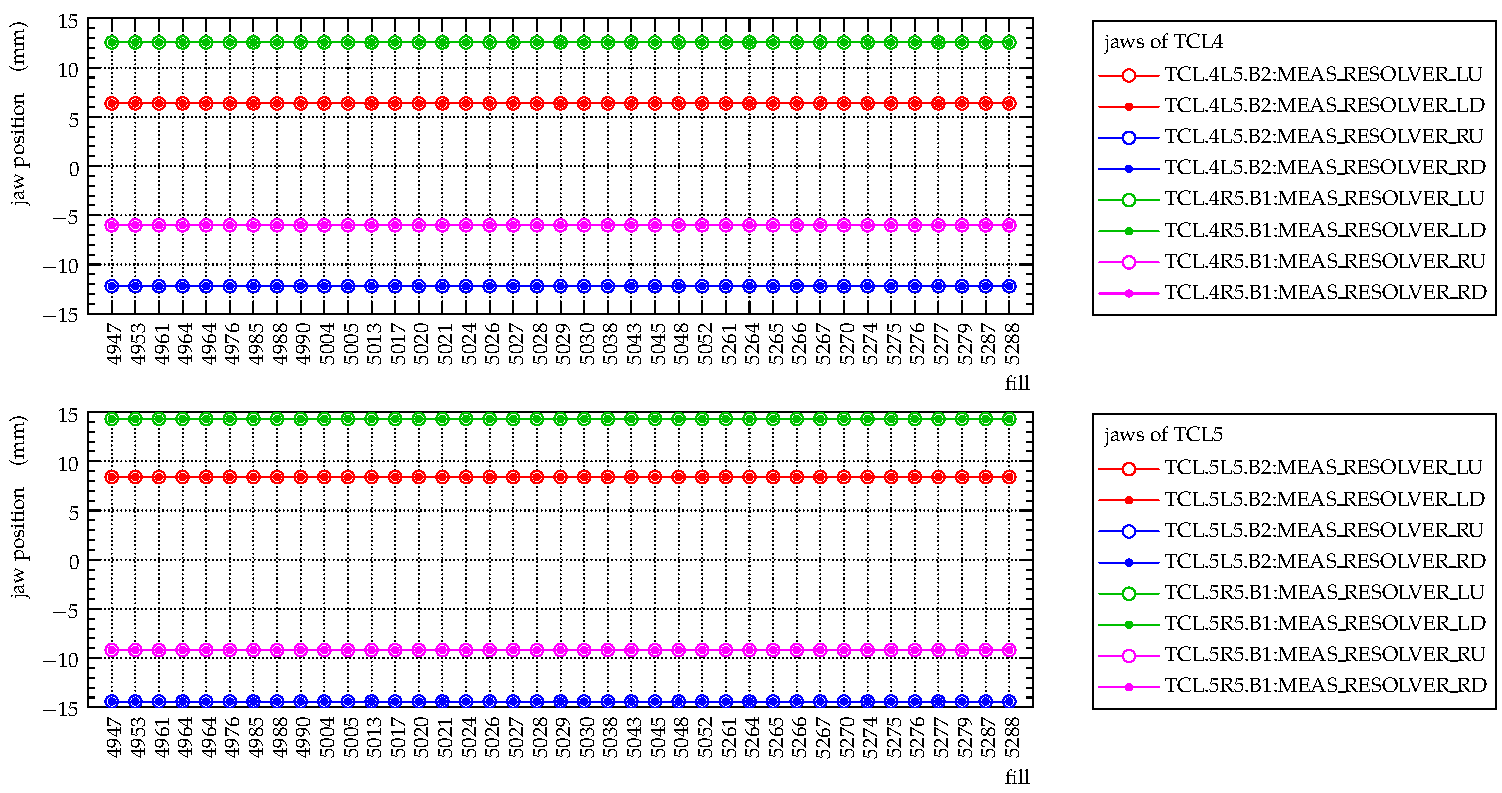
\includegraphics[width=1\hsize]{fig/conditions/collimator_positions_resolver.pdf}
\caption{%
Positions of the relevant collimator jaws as a function of LHC fill. The left/right entry for fill 4964 corresponds to the insertion with/without the safety margin. The variable names (see legend) containing B1 (B2) correspond to collimators in beam 1 (beam 2). The last two characters of the variable name indicate the jaw: L stands for left, R for right, U for upstream and D for downstream.
}
\label{fig:cond_collimators}
\end{center}
\end{figure}



%--------------------------------------------------

\subsection{Data selection}
\label{s:phys-data_selection}

The data used for the alignment come from trigger streams ``DoubleEG'', ``SingleElectron'' and ``SingleMuon''. The only reason to select these streams was their relatively high statistics. From the forward-proton point of view, all these triggers are very close to zero-bias samples.

In order to select physics protons coming from the IP, one can exploit the correlation between the horizontal hit positions in the near and far RP, as illustrated in Figure \ref{fig:hor_cuts}. This correlation can be understood from the dominance of the dispersion term in the horizontal proton-transport equation. There are two independent cuts, one for the left arm (left plot) and one for the right arm (right plot). Their effect is illustrated in Figure~\ref{fig:hor_cuts_effect}.

\begin{figure}[h!]
\begin{center}
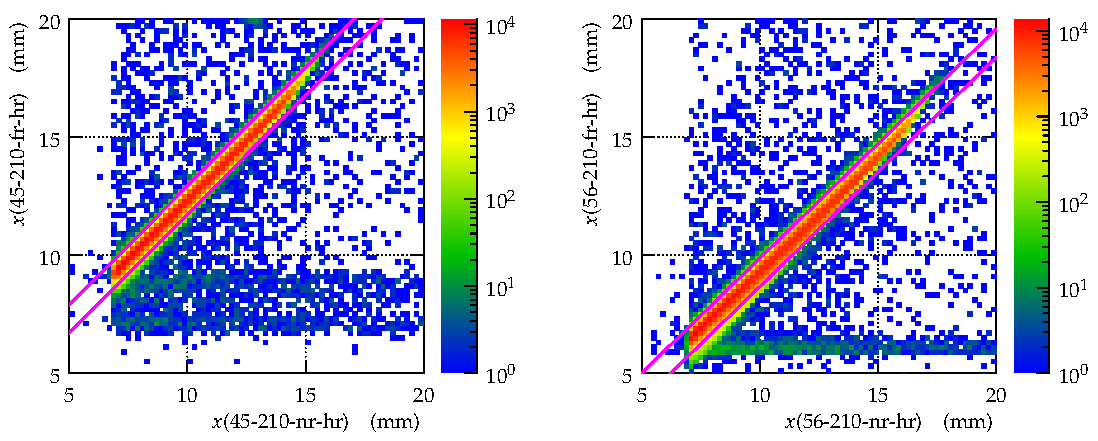
\includegraphics[width=0.7\hsize]{fig/physics_fills/hor_cuts.pdf}
\caption{%
Example of cleaning cuts, employing the correlation between the horizontal track positions in the near (horizontal axis) and far (vertical axis) RP of each station. Data from fill 4985. The magenta lines delimit the selection region, corresponding to a $3\un{\sigma}$ cut. {\it Left}: correlation in sector 45, {\it right}: correlation in sector 56.
}
\label{fig:hor_cuts}
\end{center}
\end{figure}


\begin{figure}[h!]
\begin{center}
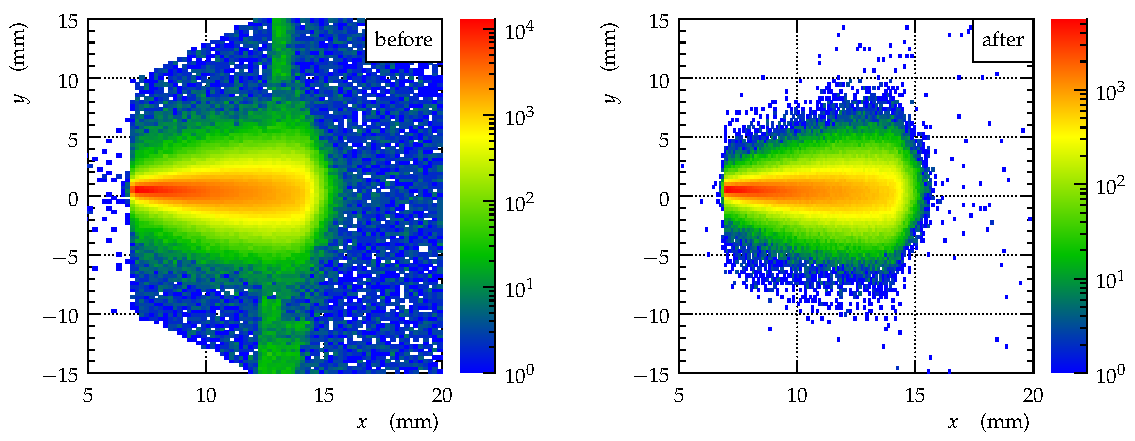
\includegraphics[width=0.7\hsize]{fig/physics_fills/hor_cuts_effect_cmp.pdf}
\caption{%
Illustration of the effect of the cleaning cuts presented in Figure~\ref{fig:hor_cuts}. Data from RP 45-210-nr-hr and fill 4985. {\it Left}: hit distribution before applying the cuts, {\it right}: the same distribution after the cuts.
}
\label{fig:hor_cuts_effect}
\end{center}
\end{figure}

Note that it would be possible to conceive a similar set of cuts in the vertical plane where the leading term in the proton transport is the one proportional to the scattering angle. However, it is more complicated due to the strong dependence of the effective length $L_y$ on $\xi$ and consequently this possibility has not been exploited so far.

%--------------------------------------------------
\subsection{Horizontal alignment}
\label{s:phys-horizontal}

The horizontal alignment is performed by matching, RP by RP, the hit distributions from a physics fill to a reference distribution from the calibration fill where the full alignment has been previously obtained by the method described in Section~\ref{s:calib}.

Figure~\ref{fig:hor_match_method} illustrates two matching metrics considered. The ``method x'' (left plot) employs histograms of horizontal track hits, $x$. The ``method y'' (right plot) uses the $x$ dependence of the standard deviation of vertical track hit, $y$.

The advantage of the ``method x'' is that it acts on distributions of $x$ which is directly related to $\xi$ (which is of primary interest for physics analyses). A disadvantage is that the histograms must be normalised (each dataset comes with different statistics) which makes the method sensitive only to distribution shapes. Another potential complication stems from radiation damage which often makes the distributions unavailable at lower values of $x$ and thus the method rely only on higher-$x$ regions which may be affected by the LHC collimators. It is thus reassuring to find the collimator positions stable over the period of interest, see Figure~\ref{fig:cond_collimators}.

The main advantage of the ``method y'' is the independence on the dataset statistics -- no normalisation is needed. A disadvantage follows from strong sensitivity to beam emittances via the beam divergence which is sizeable at this very low $\beta^*$ optics. This makes this method subject to potential fill-to-fill variations. Another complication comes from an often observed discrepancies between the calibration and physics fills in the high-$x$ region. Together with the radiation damage restricting the useful $x$ range at the low side, it shortens the lever-arm useful for alignment.

\begin{figure}[h!]
\begin{center}
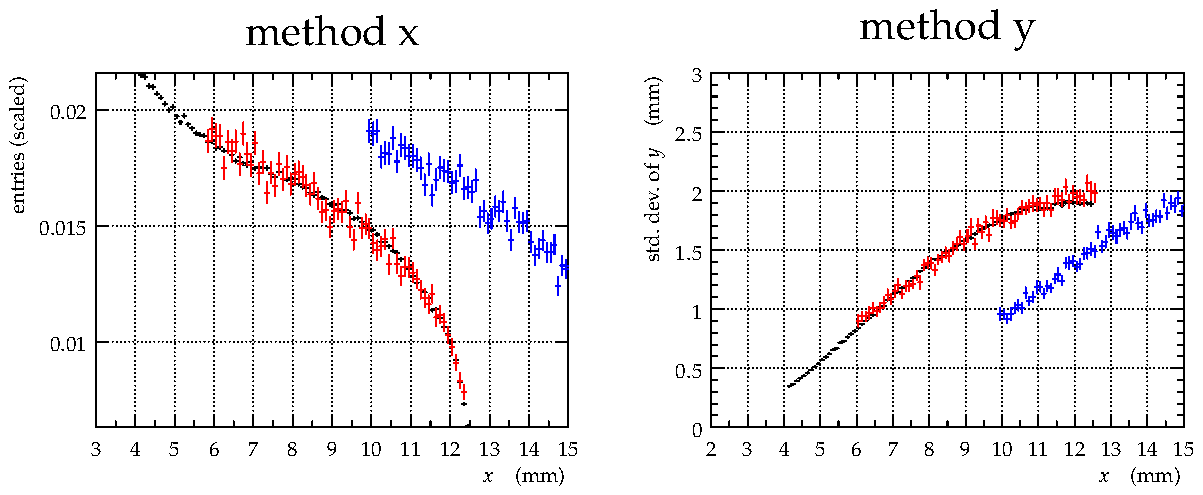
\includegraphics[width=1\hsize]{fig/physics_fills/match_method_example.pdf}
\caption{%
Illustration of the match metrics used for horizontal alignment. Black histogram: reference from the calibration fill. Blue (red) histogram: distribution from a physics fill (4964) before (after) matching.
}
\label{fig:hor_match_method}
\end{center}
\end{figure}

In a systematic study, large fill-to-fill variations were observed for the ``method y'', giving thus preference to the ``method x'' which appeared more stable. Therefore, the ``method y'' will be disregarded in what follows.

\begin{figure}[h!]
\begin{center}
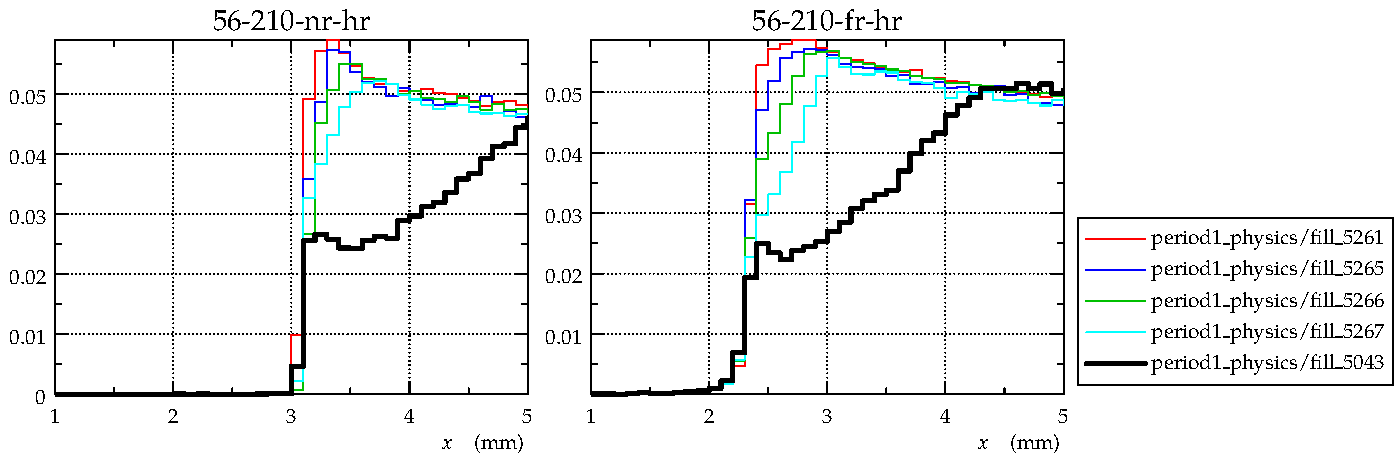
\includegraphics[width=0.9\hsize]{fig/physics_fills/x_alignment_secondary_method.pdf}
\caption{%
Illustration of the secondary horizontal alignment rule -- alignment of the histogram edge due to the sensor edge.
}
\label{fig:hor_secondary_method}
\end{center}
\end{figure}

During a systematic application of the procedure, another complication has been observed, for the RPs in the right arm and data from LHC fills $\ge 5261$. A most-likely detector inefficiency makes a systematic difference between the hit distribution from the calibration and physics fills. This inefficiency extends to rather large values of $x$, consequently making the matching range short. In order to reinforce the matching results, an additional alignment criterion has been adopted for these RPs and fills. This criterion is based on the fact that once the data in a physics fill are aligned, they can serve as alignment reference for other fills, too. Figure~\ref{fig:hor_secondary_method} shows hit distributions (black histograms) from fill 5043 (before the appearance of the problem) used as the reference for later fills (colourful histograms). The fine alignment is performed by matching the histogram edges due to the sensor edges, appearing at low-$x$ values.

The results of horizontal alignment are summarised in Figure~\ref{fig:hor_match_results}. For all RPs, the results from two data samples (red and blue points) are fully compatible. Except the RP 45-210-nr-hr which will be discussed later in Section~\ref{s:phys-left-near}, the results follow the expectations: there is about $0.5\un{mm}$ difference between the insertions with and without the safety margin and the results are stable for each insertion type.

\begin{figure}[h!]
\begin{center}
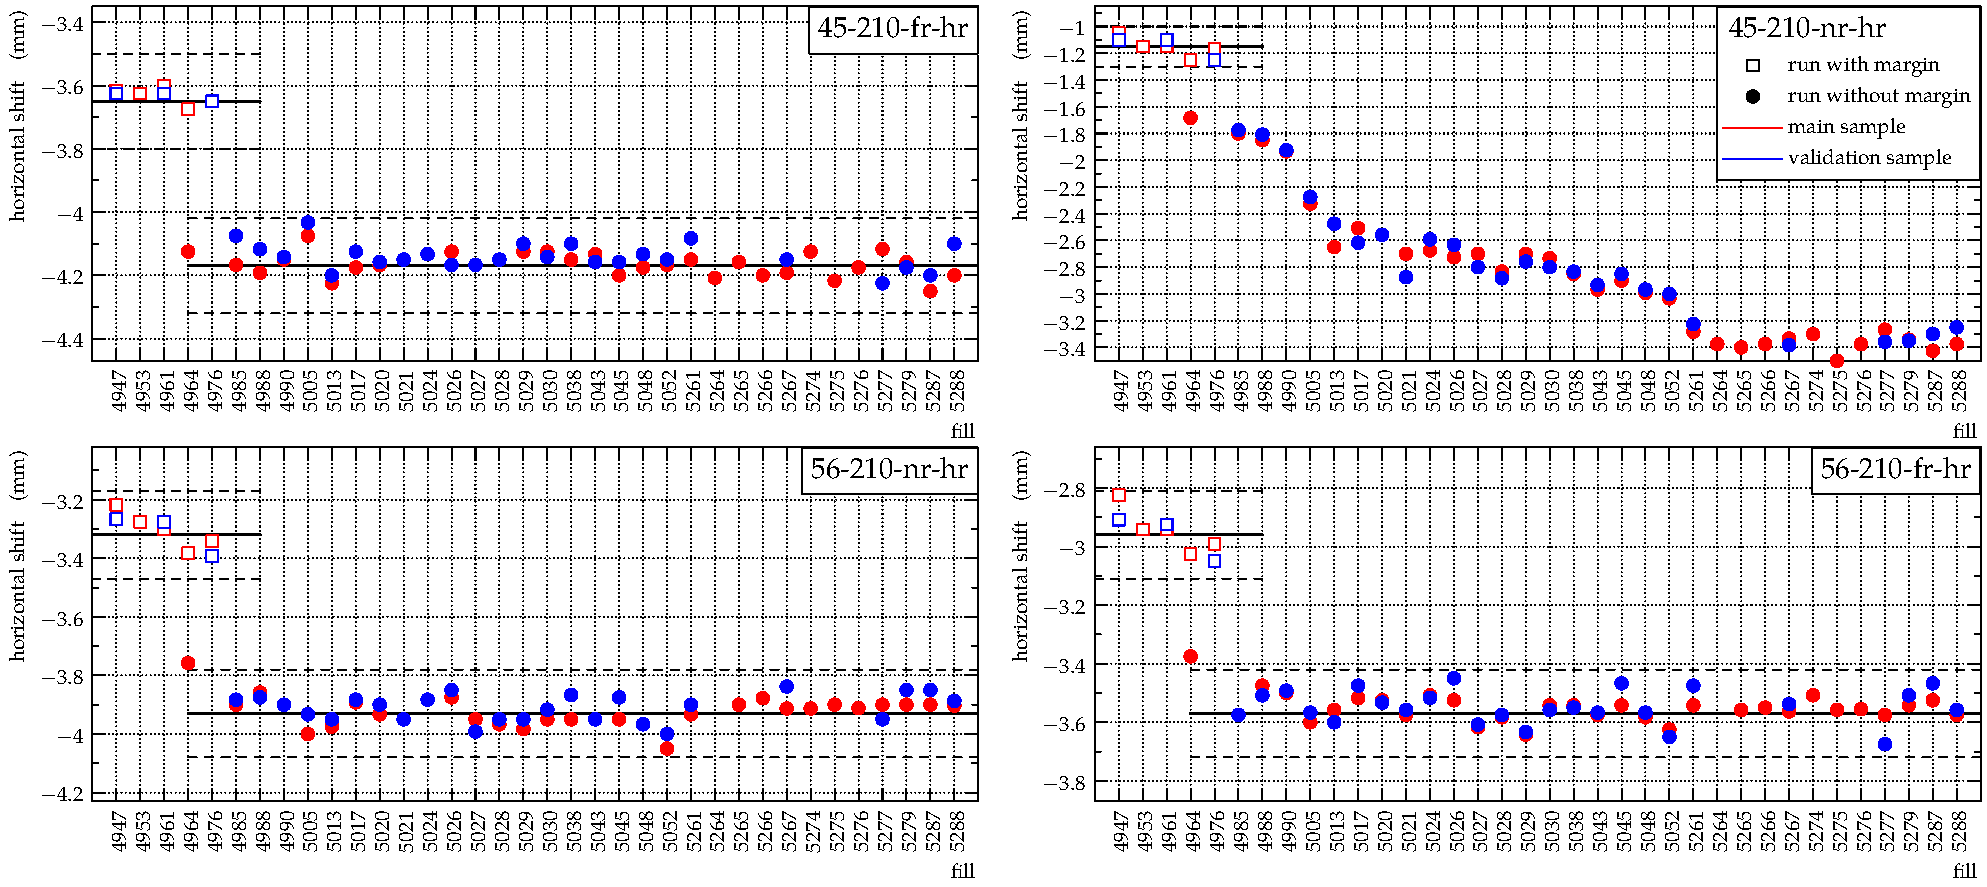
\includegraphics[width=\hsize]{fig/physics_fills/final_alignment_x_cmp_ph_sample.pdf}
\caption{%
Summary of the horizontal alignment results. Each plot corresponds to a RP. The horizontal axis indicates the LHC fill number, the vertical axis gives the correction by how much the raw hit distribution should be moved (see Figure~\ref{fig:hor_match_method}). The red and blue points represent results obtained from different data samples (CMS runs). The RP insertions with and without the safety margin are marked with hollow squares and filled circles, respectively. The horizontal black solid lines denote the means per each insertion type, the dashed lines indicate the uncertainty.
}
\label{fig:hor_match_results}
\end{center}
\end{figure}

The uncertainty of the horizontal alignment is estimated to about $150\un{\mu m}$.


%--------------------------------------------------
\subsection{Vertical alignment}
\label{s:phys-vertical}

By symmetries, the vertical position of the beam wrt.~a sensor can be inferred from the vertical ($y$) maximum of the hit distribution observed in the sensor. In contrary to the horizontal alignment, the vertical maximum is within the acceptance of the horizontal RPs. In order to be protected from backgrounds that may break the symmetries, the physics-oriented cuts from Section~\ref{s:phys-data_selection} are applied here as well.


\begin{figure}[h!]
\begin{center}
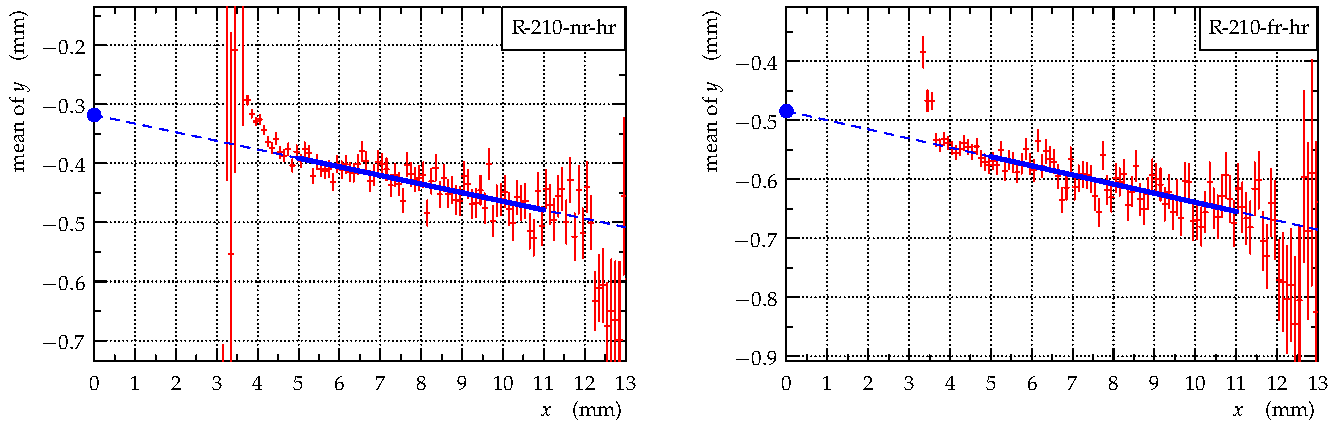
\includegraphics[width=0.8\hsize]{fig/physics_fills/y_alignment_method_example.pdf}
\caption{%
Illustration of the vertical alignment method, data from fill 4947.
}
\label{fig:vert_align_method}
\end{center}
\end{figure}



Figure~\ref{fig:vert_align_method} shows that the mean value of $y$ depends on $x$ which is unexpected. Possible origins of this tilt include
\begin{itemize}[nosep]
\item non-zero vertical dispersion, $D_y$,
\item non-vanishing $x$-$y$ coupling in the optics, e.g.~horizontal scattering angle, $\theta_x^*$, giving rise to displacement in $y$,
\item tilt of the RP in the $x$-$y$ plane.
\end{itemize}
The origin of the tilt could be studied by plotting correlations of mean of $y$, $\langle y\rangle$ vs.~$\xi$ or $\theta_x^*$.

No matter which of the above tilt origins is confirmed, the vertical alignment can be determined by the procedure illustrated in Figure~\ref{fig:vert_align_method}. After horizontal alignment, see Section~\ref{s:phys-horizontal}, the function of $\langle y\rangle$ on $x$ (red histogram) is fitted (blue solid line) and extrapolated (blue dashed line) to $x = 0$. This $y$ value (blue point) is an estimate of the beam position wrt.~the beam.

The results of vertical alignment are summarised in Figure~\ref{fig:vert_align_results}. The error bars include fit and extrapolation uncertainty, uncertainty from the horizontal alignment and uncertainty from varying the fit range. For all RPs, two data samples (red and blue) give compatible results. The RP 45-210-nr-hr exhibits a strong time-dependence and will be discussed later in Section~\ref{s:phys-left-near}. For the other RPs, the results are almost flat in time. There are minor systematic effects which can be often traced to the time variance of the tilts shown in Figure~\ref{fig:vert_align_method}. Taking this into account, the uncertainty of the vertical alignment is estimated to $150\un{\mu m}$ for the moment. Further studies are foreseen.

\begin{figure}[h!]
\begin{center}
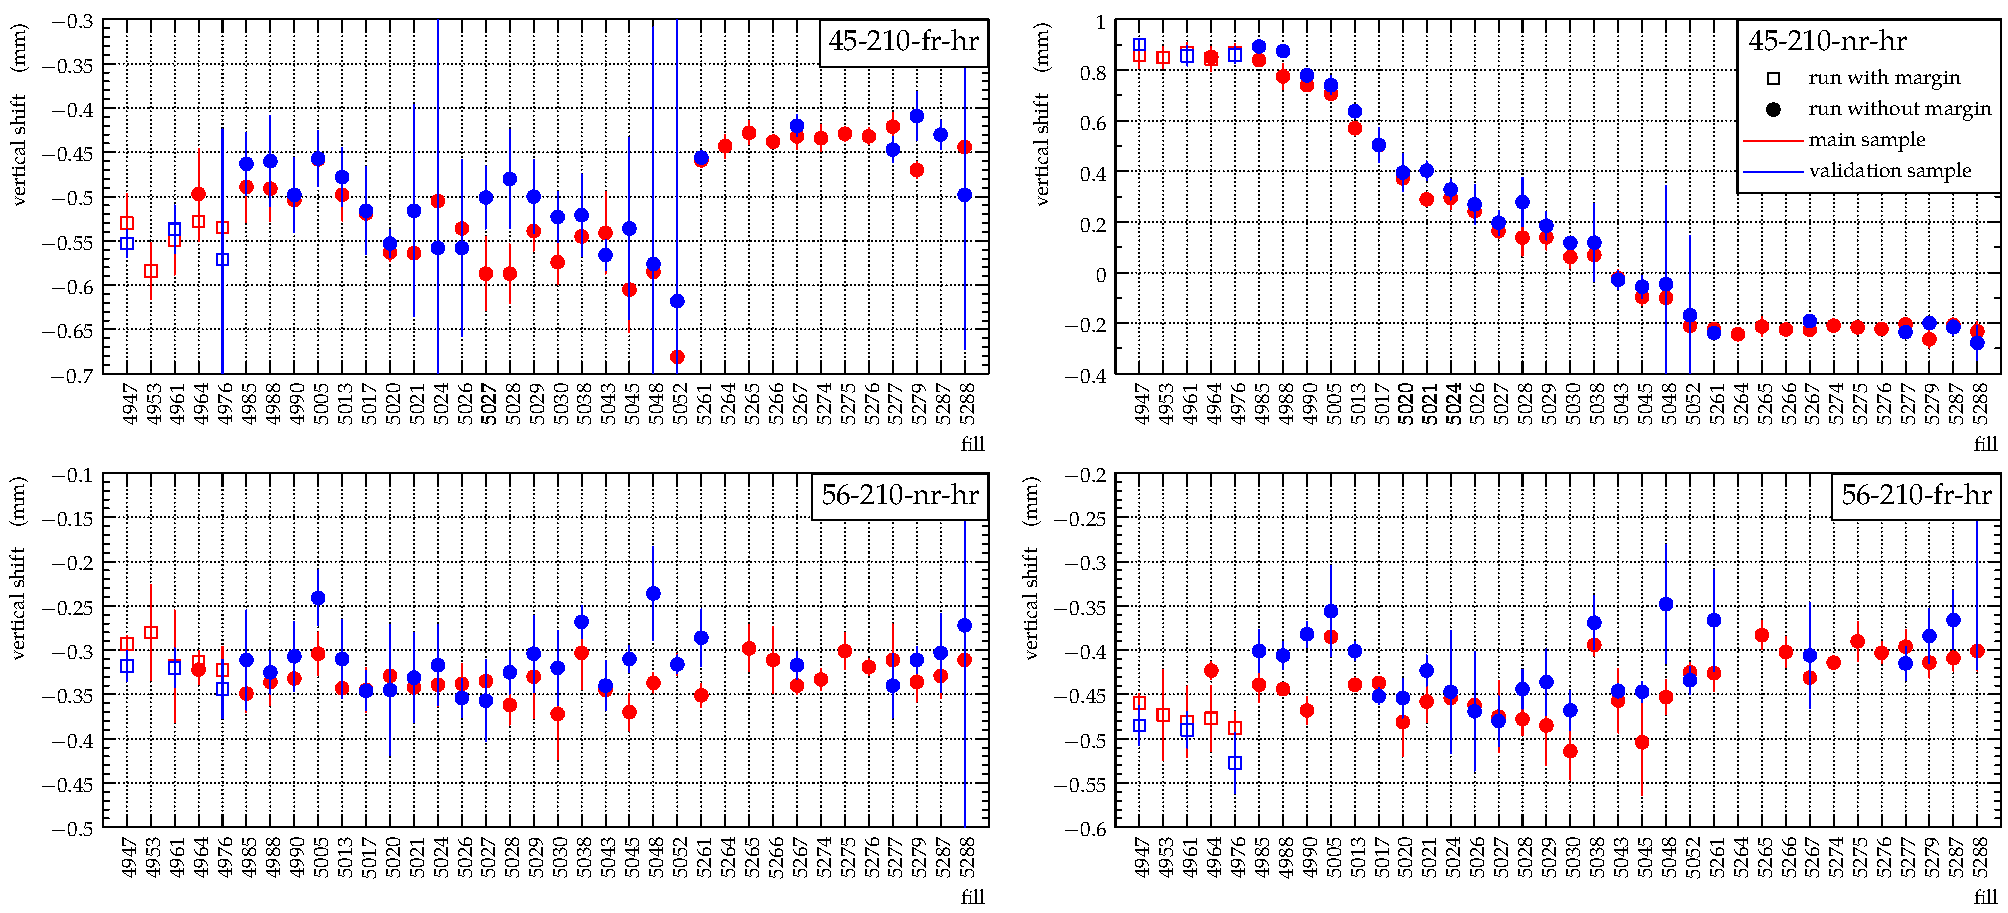
\includegraphics[width=\hsize]{fig/physics_fills/final_alignment_y_cmp_ph_sample.pdf}
\caption{%
Summary of the vertical alignment results. Each plot corresponds to a RP. The horizontal axis indicates the LHC fill number, the vertical axis gives the vertical alignment correction -- the fit extrapolation to $x=0$ as in Figure~\ref{fig:vert_align_method}. The red and blue points represent results obtained from different data samples (CMS runs). The RP insertions with and without the safety margin are marked with hollow squares and filled circles, respectively.
}
\label{fig:vert_align_results}
\end{center}
\end{figure}



%--------------------------------------------------
\subsection{RP 45-210-nr-hr}
\label{s:phys-left-near}

As anticipated above, there are indications that the sensor in the RP 45-210-nr-hr moved wrt.~the beam during the data-taking period. Figure~\ref{fig:left_near_summary} provides a correlation of these indications. The top plot is a zoom from Figure~\ref{fig:hor_match_results} and shows horizontal shift as a function of the LHC fill (ordered by increasing date). This plot indicates a shift by almost $2\un{mm}$ between the beginning and end of the data-taking period. Moreover, by comparing the data in the far and near RP in the left arm, it can be shown that the near RP was too far from the beam in the beginning and, by time, drifted to the expected position. The second plot from top is extracted from Figure~\ref{fig:vert_align_results} and describes the vertical shift -- about $1\un{mm}$ in total. The third plot from top shows the time dependence of the slopes shown in Figure~\ref{fig:vert_align_method}. The time variation is not very significant but appreciably stronger than for other RPs.

The bottom plot of Figure~\ref{fig:left_near_summary} shows mean track angles as fitted through the 10 planes of Si strip sensors. These mean angles are sensitive to RP tilts in the $x$-$z$ (green) and $y$-$z$ (magenta) planes. While for other RPs the data are compatible with no fill-to-fill variation, RP 45-210-nr-hr shows a strong fill dependence of the tilt in $x$-$z$ plane.

Overall, Figure~\ref{fig:left_near_summary} shows a strong time correlation of the four movements, starting at about fill 4988 and stopping at about fill 5264.

\begin{figure}[h!]
\begin{center}
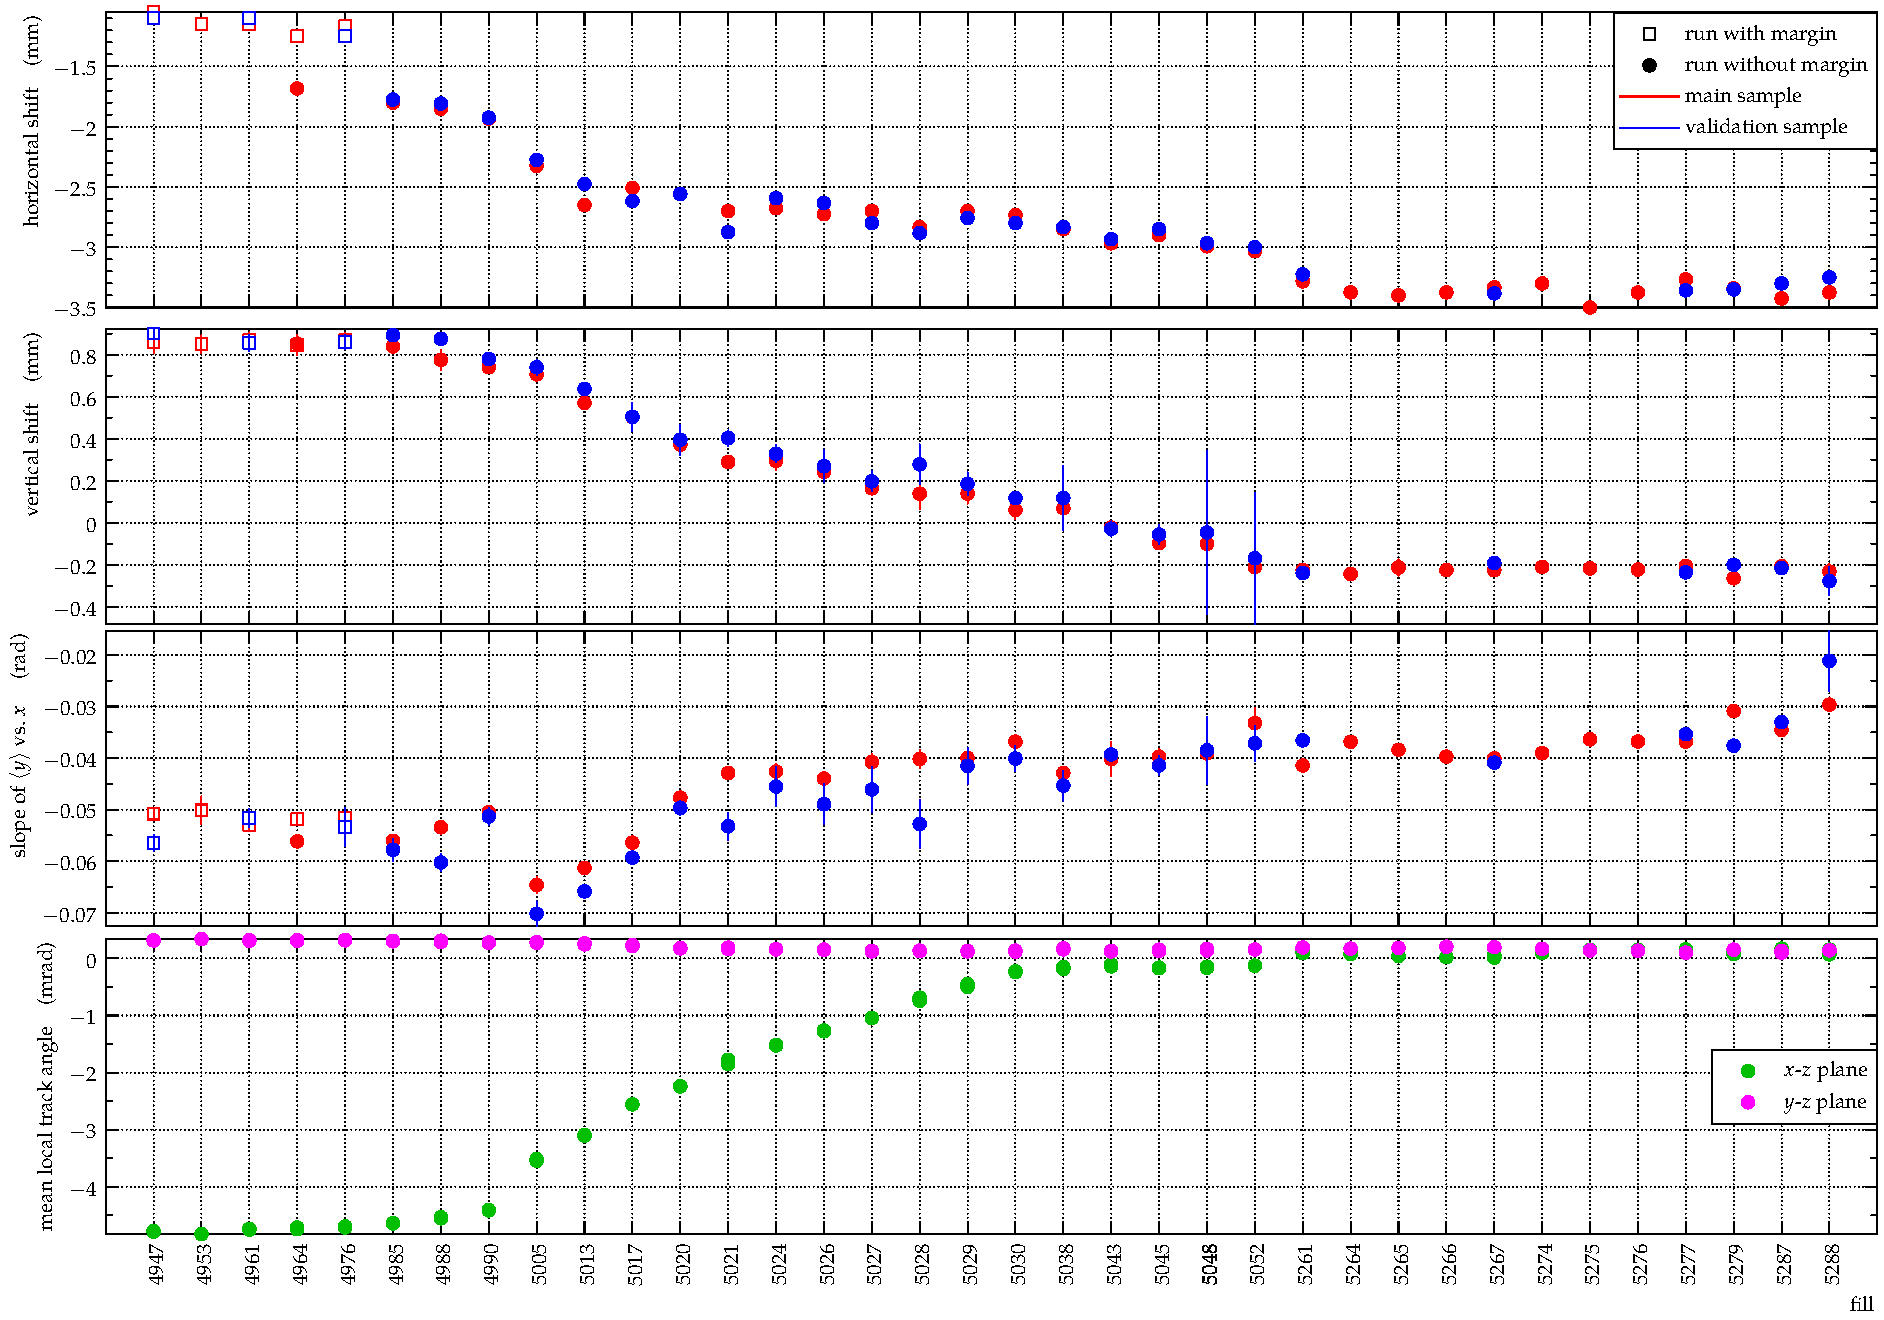
\includegraphics[width=1\hsize]{fig/physics_fills/45_210_nr_hr_summary.pdf}
\caption{%
Summary of the evidence for the movement of the RP 45-210-nr-hr. The horizontal axis, common to all plots, indicates the LHC fill number. The red and blue points represent results obtained from different data samples (CMS runs). {\it Top}: horizontal shift, {\it second from top}: vertical shift, {\it third from top}: tilt in the $x$-$y$ plane. {\it Bottom}: tilt in the $x$-$z$ plane (green) and $y$-$z$ plane (magenta).
}
\label{fig:left_near_summary}
\end{center}
\end{figure}

Since no instability has been reported by the BPMs, see Figure~\ref{fig:cond_bpm}, and since no unexpected behaviour has been observed in the far RP less than $9\un{m}$ from the near RP, it is more likely that the Si sensors moved.

Since the horizontal shift trend from Figure~\ref{fig:left_near_summary} is not reported in the RP position measurements, cf.~Figure~\ref{fig:cond_rp}, there can be only two hypotheses. First, the moving element was inside the RP (thus not affecting the RP position measurements), or second, the entire RP structure moved (both ends of the RP position gauges moved together). For the first hypothesis, it has been verified that inside the RP there is enough room for the detector package (DP) to be by $\sim 2\un{mm}$ too far out. There is a spring that should push the DP to the design position, however its force at the last $2\un{mm}$ is strongly reduced. Furthermore, visual inspection of the DP replaced in TS2 indicates some points of friction (polished surfaces). Regarding the second hypothesis, it could be that the 4 screws holding the RP structure were not taught enough.


%----------------------------------------------------------------------------------------------------

\section{Alignment and optics validation}
\label{s:val}

This section presents a simple validation of the alignment and optics calibration, based on the fact that the four RPs, in all fills, measure the same physics, up to the detector effects (acceptance, resolution, etc.). As a reference physics quantity, inclusive $\xi$ spectra will be used, see the data selection in Section~\ref{s:phys-data_selection}.

The values of $\xi$ are reconstructed per RP from the horizontal hit position, $x$, using the alignment from Section~\ref{s:phys-horizontal} and dispersion curves from \cite{optics_calibration}.

Figure \ref{fig:xi_cmp_run} shows an event-by-event correlation of $\xi$ values reconstructed in the near and far RP of the left spectrometer arm. As expected, the correlation is very close to the dashed line representing equality of both $\xi$'s.


\begin{figure}[h!]
\begin{center}
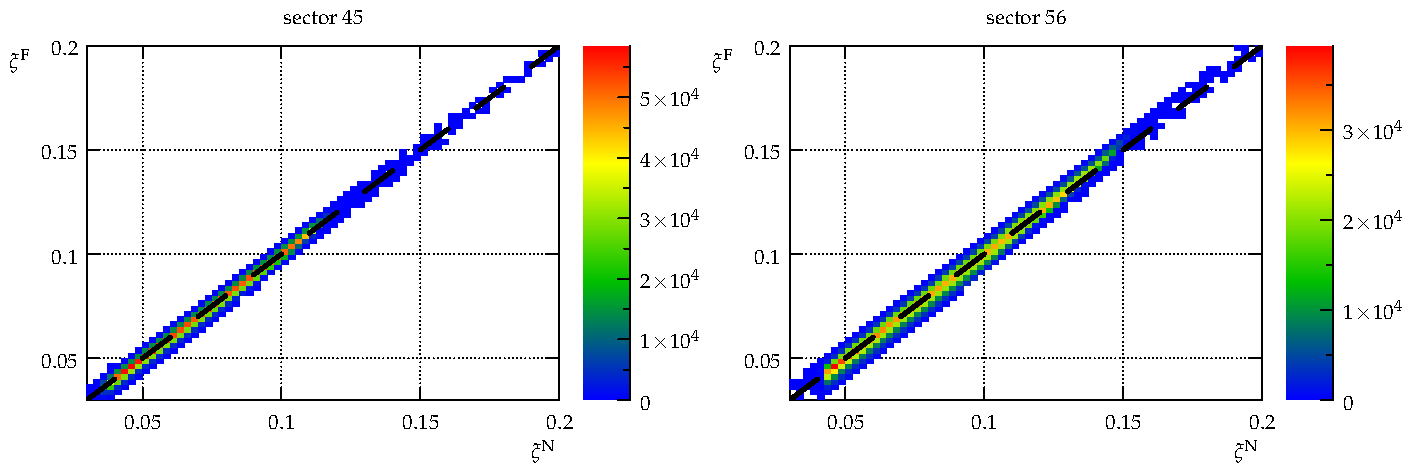
\includegraphics[width=\hsize]{fig/validation/xi_NF_corr_cmp.pdf}
\caption{%
Example of correlation of $\xi$ values reconstructed in the near (horizontal axis) and far (vertical axis) RP. Data from run 5261. {\it Left}: sector 45, {\it right}: sector 56.
}
\label{fig:xi_NF_cmp}
\end{center}
\end{figure}


Figure \ref{fig:xi_cmp_run} compares the $\xi$ distributions from several fills but the same RP. Apart from the lower-$\xi$ regions affected by the radiation damage, there is a very good overlap with the thick black histogram originating from the calibration fill. This manifests the stability of the calibration procedures.


\begin{figure}[h!]
\begin{center}
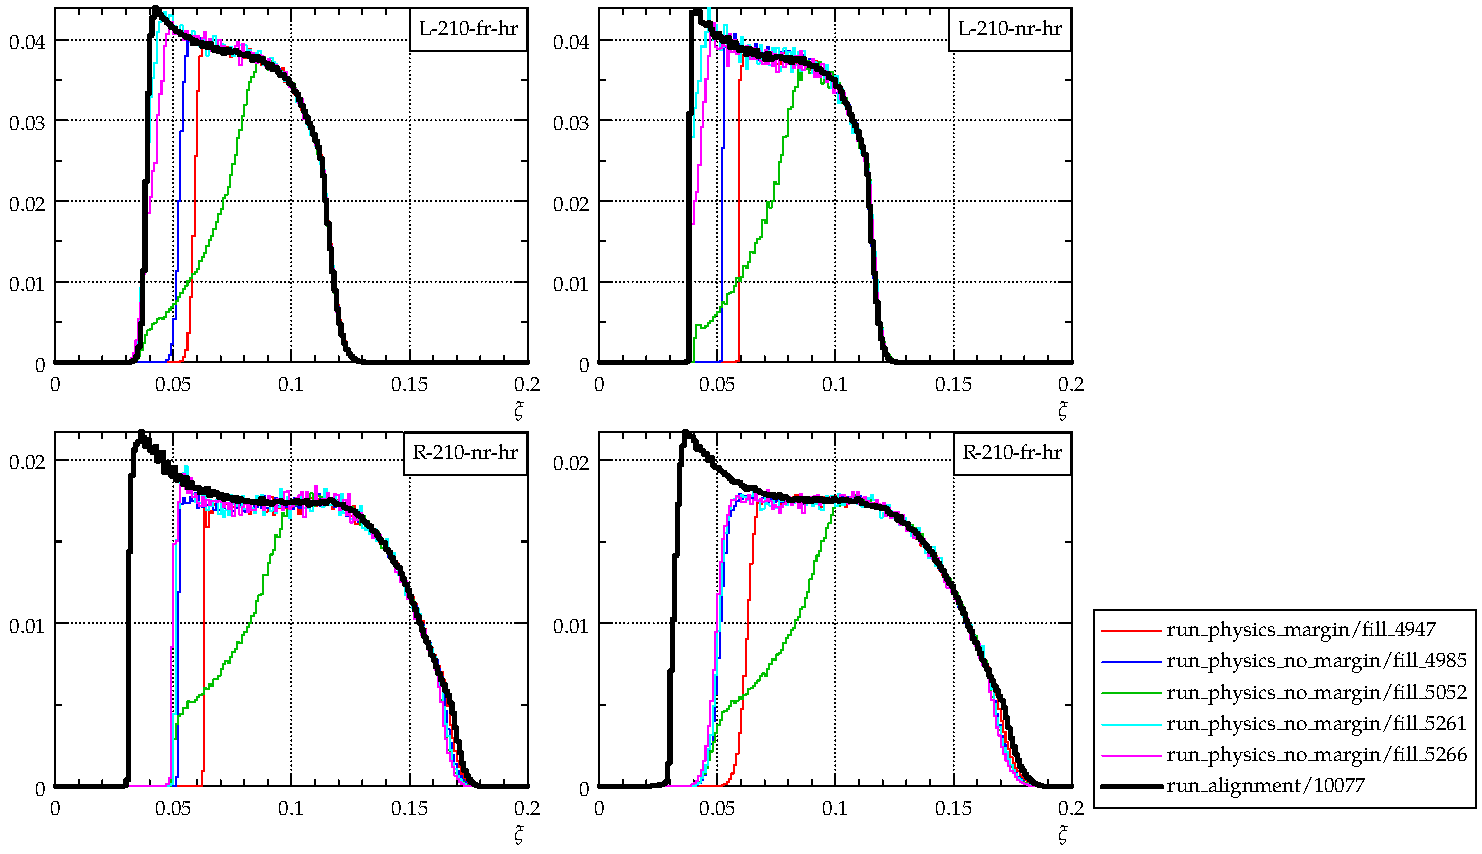
\includegraphics[width=\hsize]{fig/validation/xi_cmp_run.pdf}
\caption{%
Fill-to-fill comparison of $\xi$ distributions extracted from single RPs. The green and magenta curves exhibit a strong impact of the radiation damage at lower values of $\xi$, effectively equivalent to inefficiency.
}
\label{fig:xi_cmp_run}
\end{center}
\end{figure}


Figure \ref{fig:xi_cmp_rp} compares the $\xi$ distributions from the same fill but different RPs. In the left plot (calibration fill), disregarding the region $\xi\gtrsim 0.08$ affected by acceptance limitations, one can observe a good shape agreement among the histograms from all the four RPs. In the physics fills (middle and right plot), the common $\xi$ region unaffected by detector effects is too short for drawing a conclusion. However, the fill-to-fill stability shown in Figure~\ref{fig:xi_cmp_run} allows for extrapolating the agreement from the calibration fill to the physics fills, too.

\begin{figure}[h!]
\begin{center}
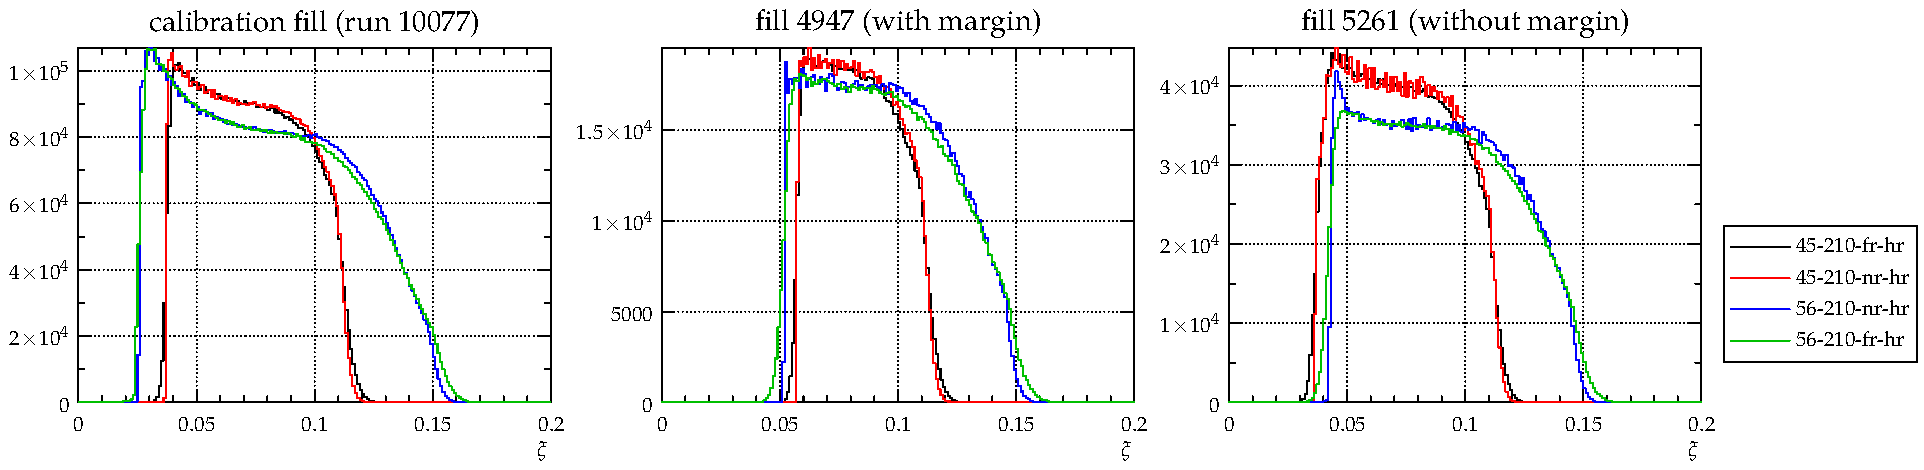
\includegraphics[width=\hsize]{fig/validation/xi_cmp_rp.pdf}
\caption{%
Comparison of $\xi$ distributions from different RPs. The 3 plots correspond to 3 selected fills, see captions.
}
\label{fig:xi_cmp_rp}
\end{center}
\end{figure}



%----------------------------------------------------------------------------------------------------

\section{Summary}
\label{s:sum}

The first alignment of CT-PPS detectors has been achieved by a two-stage procedure. In the first stage, the alignment was performed with data from a special calibration fill, where both horizontal and vertical detectors were inserted close to the beam. In the second stage, the alignment information was transferred to the physics fills with high intensity and only horizontal RPs inserted.

The alignment in the calibration fill employs the standard ``TOTEM'' procedure and reaches precision of $5\un{mrad}$ for tilts ($x$-$y$ plane), $50\un{\mu m}$ for horizontal shifts and $75\un{\mu m}$ for vertical shifts.

The horizontal alignment in physics fills is achieved by matching physics hit distributions to the reference from the calibration fill. The estimated uncertainty is about $150\un{\mu m}$.

The vertical alignment follows the horizontal one and is based on profile histograms of mean $y$ as a function of $x$. These histograms exhibit unexpected tilts, the origin of which is yet to be studied. Irrespective of the origin, the alignment is extracted by extrapolating the profiles to $x=0$ which estimates the vertical beam position wrt.~the sensor. The uncertainty estimate is about $150\un{\mu m}$. A part of the uncertainty stems from systematic fill-to-fill differences that can be traced back to instability of the tilts of the profile histograms.

Many unexpected results have been obtained for the RP 45-210-nr-hr, including horizontal and vertical shifts and tilts in $x$-$y$ and $x$-$z$ plane. All these observations are strongly correlated in time and hint that the sensors moved during the data-taking period. A hypothesis reads that the detector package moved within the RP, another hypothesis states that the entire RP structure was loosely attached to the support frame. In any case, the offline alignment procedure above is able to track the movements and provide fill-dependent alignment corrections.

As a combined validation of alignment and optics calibration, consistent inclusive $\xi$ distributions have been obtained from different RPs and different fills, compatible with the assumption that all RPs measure the same physics irrespective of the LHC fill.

%----------------------------------------------------------------------------------------------------

\begin{thebibliography}{99}

\bibitem{optics_calibration}
	Note being written by Frici.

\bibitem{rp-names}
	Product breakdown structure and naming scheme of the Roman Pot System, EDMS document,
	\url{https://edms.cern.ch/document/906715/0.7}.

\bibitem{totem-ijmp}
	\Name{G.~Antchev \etal{}~(TOTEM Collaboration)}
	\Review{Int.~J.~Mod.~Phys.~A}{28}{2013}{1330046}.

\bibitem{jan_thesis}
	\Name{J.~Ka\v spar}
	PhD Thesis, CERN-THESIS-2011-214,
	\url{http://cdsweb.cern.ch/record/1441140}.


\bibitem{totem-8tev-90m}
	\Name{G.~Antchev \etal{}~(TOTEM Collaboration)}
	\Review{Nucl.~Phys.~B}{899}{2015}{527-546}

\iffalse

\bibitem{totem-jinst}
	\Name{G.~Anelli \etal{}~(TOTEM Collaboration)}
	\Review{JINST}{3}{2008}{S08007}.
    %The TOTEM Experiment at the CERN Large Hadron Collider, JINST 3 S08007, 2008

\fi

\end{thebibliography}

\end{document}
